%\documentclass[twoside,agupp]{aguplus}       % PREPRINT
%\documentclass[jgrga]{aguplus}              % CAMERA-READY, JGR
%\documentclass[agums,10pt]{aguplus}         % MANUSCRIPT

%\documentclass[grlga]{aguplus}              % CAMERA-READY, GRL, single col
\documentclass[agupp]{aguplus}              % CAMERA-READY, GRL, double col

%----------------------------------------------------------------------
%\usepackage[expert]{lucidabr}
\usepackage{graphicx}
\usepackage{xspace}
\usepackage{subfigure}

%\usepackage[T1]{fontenc}
%\usepackage[expert]{lucidabr}
%\usepackage[utf8]{inputenc}

\DeclareGraphicsExtensions{.pdf,.jpg,.png,.eps}
\usepackage[usenames]{color}

%\usepackage{pdfdraftcopy}

%% Shortcuts
\newcommand{\kc}{\tetsf{kCARTA}\xspace}
\newcommand{\wn}{cm$^{-1}$\xspace}
\newcommand{\um}{$\mu m$\xspace}
\newcommand{\gn}{\textsf{GENLN2}\xspace}

\newcommand{\ch}{CH$_4$\xspace}
\newcommand{\wv}{H$_2$O\xspace}
\newcommand{\cd}{CO$_2$\xspace}
\newcommand{\ozone}{O$_3$\xspace}
\newcommand{\nit}{N$_2$O\xspace}
\newcommand{\co}{CO\xspace}
\newcommand{\so}{SO$_2$\xspace}
\newcommand{\hno}{HNO$_3$\xspace}


\newcommand{\mydeg}{\mbox{$^\circ$}}

\newcommand{\dlandgraph}[3]
   {
   \begin{center}
   \includegraphics[width=#1\semwidth,height=!]{#2}   
   \includegraphics[width=#1\semwidth,height=!]{#3}   
   \end{center}
   }

% Good options
\printfigures           
\doublecaption{35pc}    
\sectionnumbers         
\extraabstract          

\lefthead{S. DeSouza-Machado et.\ al.}
\righthead{AIRS vs NWP}
%\received{May xx, 2006}
%\revised{June xx, 2007}
%\accepted{July xx, 2008}

\slugcomment{Submitted to Journal of Geophysical Research}

\begin{document}

\title{Using two Cloud-Representation Models to make statistical comparisons
between AIRS infrared radiance observations and calculations simulated using
Numerical Weather Prediction fields}

\author{S. G. DeSouza-Machado, L. L. Strow, S. E. Hannon, C. Hepplewhite, \newline P. Schou, A. Tangborn}
\affil{JCET/Physics Department, University of Maryland
  Baltimore County, Baltimore, Maryland}
\author{X. Huang, X. Chen} 
\affil{University of Michigan, Ann Arbor, Michigan}
\author{X. Liu} 
\affil{NASA Langley Research Center, Langley VA}

\begin{abstract}
\small 

We use radiative closure to assess global 0.125 \mydeg resolution
Numerical Weather Prediction (NWP) forecasts from the European Center
for Medium Range Weather Forecasting (ECMWF) model, using one full day
of all-sky infrared radiances measured by NASA's Atmospheric Infrared
Sounder. The conversion from NWP model fields to radiances is
accomplished using two different cloud representation models, which
are the Maximum Random Overlap model and a fast accurate TwoSlab Cloud
model we have recently developed. The radiative closure comparisons
enable us to assess the physics parametrizations used to produce
geophysical fields, by focusing on the AIRS 1231 \wn channel for
comparing probablility distribution functions (pdfs) of the clear-sky
and all-sky observations and calculations. The 0.125 \mydeg grid
resolution approaches the AIRS footprint size, and over the ocean,
scenes that are carefully screened as being cloud-free show a high
degree of consistency between observations and the forward
models. Similar examination from the cloud-contaminated cases also
show very high consistency between the two cloud-representation models
: for example when used with the ECMWF model fields, both cloud
representation/scattering models produce fewer Deep Convective Clouds
(DCC), and warmer Brightness Temperatures (BT) for Marine Boundary
Layer (MBL) clouds, than observed. Night time clear sky biases for a
spanning set of 41 AIRS channels are typically less than 0.5 K over
the ocean, except for the ozone sounding channels where the biases can
be as large as -1.5 K, and average to a $\sim$ 10\% ozone columnn
deficiency. The average cloud forcing (converted to BT differences)
for night time all-sky ocean scenes is on the order of 10 K in the
tropics and 13 K in the midlatitudes. Night time all-sky biases
average to be on the order of 1 K in the longwave (6-15 \um) AIRS
spectrum, and larger in the shortwave (3-4 \um) region, suggesting the
TwoSlab scattering algorithm is less accurate in the shortwave.

\end{abstract}

\begin{article}

\section{Introduction}

Numerical Weather Prediction (NWP) models assimilate data including that 
from radiosondes  and observations from orbiting microwave
and infrared instruments, in order to initializate the dynamical
models from which weather predictions are made. The underlying
physical based parametrizations in NWP models are also used in climate
codes, and indeed NWP models have progressed to the extent that the
re-analysis output could arguably be used for climate studies
\citep{dee:11*1}. However since the atmosphere, ocean and the land
surface exhibit complex behavior over large temporal and spatial
scales, the physics in the NWP models is limited by the inherent
pameterization of subgrid processes, including and especially clouds
which are a critical component of radiative forcing. In addition
instrumental drifts affect the assimilated data while updates to
the model physics parametrization can affect the output geophysical
fields \cite{mor:91, sau:13}.

These reasons underline the importance of both validating the physics
of the NWP models and to monitor the stability of the observational
data. Weather observations can be divided into conventional- and
satellite- based. Conventional \emph{in-situ} observations include
those from surface (land, ship and buoy) stations, and from aircraft
and balloons. These are very localized and lead to a non-uniform
concentration as they are mostly obtained on or over continents,
typically twice a day.

Conversely instruments on board Earth-orbiting satellites routinely
provide global measurements on time scales ranging from almost
continuous (geostationary) to roughly twice daily (polar
orbiting). Since the early 2000's, a number of high spectral
resolution, low noise, very stable new generation microwave (MW) and
infrared (IR) sounding instruments have been deployed on board Earth
orbiting satellites, which provide Top of the Atmosphere (TOA)
radiance observations obtained over both cloud-free scenes (clear-sky)
and cloud-contaminated (all-sky) scenes. While the TOA radiances
measured by these sounders contain information related to atmospheric
gases and clouds, the radiances cannot be compared directly to the NWP
model fields. Instead the comparisons need to be made either by using
the satellite measurements for physical retrievals which complement
\emph{in-situ} measurements obtained at conventional sites, or by
using the NWP fields together with a radiative transfer model for
radiative closure comparisons. Either of these comparisons would be
affected by the accuracy and resolution of the measured radiances, and
by other factors described below.

The information retrieved from TOA radiances must be carefully
interpreted, as the inversion of radiance contributions summed along
the viewing path is an ill-posed problem : multiple atmospheric
constituents at all layers contribute to these radiances, each having
their own uncertainties. Especially for infrared sounders, accounting
for cloud contamination adds to the retrieval complexities.
Conversely, the same IR hyperspectral radiance data can be used to
probe current state-of-the-art NWP model fields and diagnose
parametrization schemes in the models \citep{she:13} via radiative
closure, provided one has an accurate scattering-based radiative
transfer code. On an individual observation pixel basis, one may be
vulnerable to time and spatial mismatches between the model field
outputs and observations, necessitating statistical comparisons using
probability distribution functions.  Analyzing all-sky scenes should
yield valuable information, since clouds need to be represented
accurately as they are key elements of the water and energy cycles and
play an important role in atmospheric dynamics and thermodynamics
\citep{kok:11}. Clouds also affect both reflection of solar radiation
(cooling) and trapping of outgoing longwave radiation (warming).  For
example low clouds such as Marine Boundary Layer (MBL) cloud decks
typically have a cooling effect since they are close to the surface
but reflect sunlight, while high thin cirrus tends to have a warming
effect as they are transparent to shortwave radiation but trap
outgoing infrared radiation and re-radiate it downwards; conversely
Deep Convective Clouds (DCC) have both cooling and warming effects
which though large, cancel each other out.

A recent study monitored 3 years of clear-sky satellite biases using
radiances computed with NWP fields \citep{sau:13}. NWP schemes can
discard upto 75\% of the datellite data \cite{bau:10} due to unknown
emissivity (land,ice,snow) and cloud contamination, the latter due to
difficulties in fast accurate modelling of radiative transfer through
clouds as well as to NWP cloud and moisture parameterization
deficiencies. This paper uses radiative closure to compare one day's
worth of high quality observational IR all-sky radiance dataset
against radiances computed using NWP geophysical and cloud fields
(both analysis and forecast) in two different cloud representation
schemes. Key considerations are the accuracy and computational speed
of the cloud scheme within the radiative transfer model(s) - modeling
horizontal inhomogeneties of clouds requires multiple streams to
simulate overlapping clouds extending vertically through the
atmosphere, placing heavy computational burdens on any
radiative transfer model.

Data from the Atmospheric Infra-Red Sounder (AIRS) \citep{str:02*1} is
used in this paper. AIRS was designed to provide improved temperature
and humidity profiles for numerical weather prediction and long-term
climate studies. Detectors spanning the 650 to 2700 \wn (or 3.7 to 15
\um) spectral region make AIRS radiances sensitive both to the
underlying geophysical state of the atmosphere (temperature, humidity,
ozone and trace gas constituents and surface parameters)
\citep{aum:02*2,str:02*2}, as well as to ice and water clouds
\citep{kah:03*1,kah:05*1,wu:09}. The radiances are also sensitive to
large aerosol particles such as mineral dust and volcanic ash
\citep{mac:10,cla:10}, though their effects are not considered here.

The NWP model assessed is that used by the European Center for Medium
Range Weather Forecasts (ECMWF). This center provides operational
medium- and extended-range forecasts at a high vertical and grid
resolution output; a more stable re-analysis output (run $\sim$ 3
months later) is also available on a coarser grid.  The center uses a
meteorological global forecasting model on synoptic scales run
every 12 hours.  We also study some aspects of the cloud
and moist convection parametrizations, by assessing observations against 
radiances computed using the cloud and geophysical NWP fields.

The rest of the paper is organized as follows. After describing the
AIRS instrument and the ECMWF model, the paper then describes the RT
models and cloud representation schemes used in the paper; using the
ECMWF NWP fields we examine the statistical differences in the output
of these RT codes. We then present statistical comparisons
between observations and radiative transfer calculations for March
11,2011, a randomly chosen typical day. A discussion of the
information content of AIRS radiances in the presence of clouds, and
perturbations to one of the cloud representation schemes, are also
presented. We finish by studying regions of shallow convection MBL clouds
and DCC clouds, and use some of the available geophysical NWP
variables as an aid to probe differences in the observations compared
to the RT calculations in AIRS data granules containing these clouds.

\section{Description of the Instrument, NWP Model fields and simulation code}

\subsection{The AIRS instrument and data} The Atmospheric Infrared
Sounder (AIRS) on board NASA's polar orbiting EOS/Aqua platform has
2378 channels, covering the spectral range 649-1136, 1217-1613,
2181-2665 \wn. The full widths at half maximum satisfy $\nu/\delta\nu
\sim 1200$, with the noise equivalent change in temperature $(NE
\Delta T)$ $\le$ 0.2K.  The instrument became operational in September
2002, has performed beyond its requirements, and is expected to last
at least another 5 more years.  

AIRS has a 13.5 km nadir footprint from a $\sim$ 705 km orbit, and its
radiances have been shown to be very stable and accurate
\citep{aum:06}. A few AIRS detectors have deteriorated over time,
reducing the available pool of channels to study. Many AIRS channels
have similar weighting functions, making it un-necessary to compare
observations versus simulations for all 2378 channels. In this paper
we mainly focus on AIRS channel 1291 (centered at 1231 \wn with a
width of about 1 \wn), which is in the thermal infrared window
region. The window channel clear sky weighting
functions peak near the surface, as the clear sky atmospheric
absorption is dominated by the water vapor continuum, weak water lines
and lines due to some trace gases. In between the water lines, the
total absorption is least in the 961 and 1231 \wn region (AIRS
channels 903 and 1291). We chose Channel 1291 (1231 \wn) since it has
less cloud/aerosol interference than Channel 903, and also because for
column amounts of water larger than about 30 mm, the water amount
dependance of the continuum coefficients means this channel has less
water contamination than Channel 903.  AIRS channel number 2333
centered at 2616 \wn has even less water vapor contamination, but is
avoided since the simulated radiances additionally depend on an
accurate knowledge of scattering phase functions, required to model
solar scattering from clouds and aerosols.

AIRS data are distributed in 6 minutes granules (10 per hour),
yielding a total of 240 granules per day. Each granule consists of 90
cross track observations (spanning about $\pm$ 49.5 degrees from nadir),
with a total of 135 scan lines along the orbit track, yielding about
2.92 million observations in a single 24 hour period. The Aqua
satellite orbit provides many more observations over the poles than
the tropics, so where necessary we subsample the data using a
\emph{cos($\theta_{latitude}$)} weighting, especially when considering
global statistics. A publicly available AIRXBCAL Level 1B
calibration subset includes clear scene matchup based on scene
homogeneity and comparisons of BT1231 observations to NWP surface
temperatures \citep{aum:07}. Typically this prunes away about 98-99\%
of the daily AIRS observations.

\subsection{The ECMWF model fields}
\label{ECMWF_cloud}

The core ECMWF 0-10 day forecasts are
produced using the Integrated Forecasting System (IFS), which has 5
component models (see for example http:// www.ecmwf.int/ about/
forecasts.html). Details can be found in the user
guides found in http://www.ecmwf.int/research/ and in the IFS
documentation, and are summarized in the next two paragraphs using
information from \citep{upp:05,dee:11*2}.

The model accounts for the effects of a number of different physical
processes such as short-wave and long-wave radiation, convection and
clouds; subgrid scale cloud effects are handled via parametrization.
The uppermost level is typically 0.01 mb, with 91 terrain following
$\sigma$ levels from the surface to this pressure level. The pressure
level spacing is finest in the boundary layer and coarsest at the top,
while the model timestep is 10 minutes. The convection parametrization
scheme is based on \citep{tie:89} and does not predict individual
convective clouds, but on a cell by cell basis models the physical
effects such as momentum and energy transport to allow one of deep,
shallow or mid-level convection. Clouds are handled by
explicit equations for amount and cloud cover;
radiation is divided into longwave and shortwave components and
interaction with clouds is modeled using a cloud overlap algorithm.

We use the ECMWF higher resolution (0.125\mydeg) output grid fields
instead of the coarser but more temporally stable re-analyses fields,
as we want the closest spatial match to the AIRS
observations. The 0.125\mydeg horizontal grid resolution is about 14
km at the equator, approximately the same size as the 13.5 km AIRS
nadir footprint. The geophysical, cloud and other fields are globally
represented using a spherical harmonic expansion truncated at
T1279/16km. The assimilation algorithm is 4DVAR, with observational
data assimilated into the model in 12 hour windows. NWP fields are
output at synoptic hours 0000, 0600, 1200 and 1800 UTC; outputs at
0000 and 1200 hours are analyses from ingesting global observations
such as radiosonde and satellites, while the 0600 and 1800 hour
outputs are also analyses but from a more limited set, mainly to
stabilize the output. The 0300 and 0900 hour outputs, and 1500 and
2100 hour outputs, are forecasts extrapolated from the 0000 and 1200
hour analysis.

AIRS is on a 1:30 pm equator ascending overpass orbit while ECMWF
analyses/forecast are output at 3 hour intervals (8 per day) starting
at 00.00 GMT.  The closest in time and space geophysical parameters
are matched to each AIRS observation, using the AIRS L1B ground
observing geolocation points.  This means the profile versus observed
(latitude,longitudes) matchups are within 0.125\mydeg $\pm$ 0.05\mydeg
of each other, while the time differences are al,ost uniformly
distributed within $\pm$ 1.5 hours. We ingest the NWP
set of geophysical parameters, integrates the water vapor and ozone
point profiles (typically in ppmv or g/g) over a finer grid and saves
the resultant layer averages (in molecules/cm2) as input to SARTA. We
can also adjust profiles of an additional handful of "variable"
atmospheric gases such as carbon dioxide (\cd), nitrous oxide (\nit),
carbon monoxide (\co), methane (\ch), sulphur dioxide (\so), and
nitric acid (\hno); the profiles for other radiatively minor "fixed"
gases such as chloro-fluoro-carbons (CFCs) come from a US Standard
Profile.

\subsection{Radiative Transfer Models}

Two different radiative transfer algorithms (RTA) used to simulate
infrared radiances for the AIRS instrument. One uses two cloud slabs
while the other uses clouds at all layers. Both models are designed
for speed and accuracy needed in operational retrievals, where the
atmosphere is represented within the AIRS 100 pressure layer scheme
\citep{str:02*2}; layer thicknesses range from 0.25 km at the surface,
0.75 km at the upper tropopause, and about 4 km at 82 km, which is the
top level (TOA) for the model.

The first RT model is the Stand Alone Radiative Transfer Algorithm
(SARTA). The clear sky version (with gray cloud capability) is used in
the NASA AIRS Level 2 retrievals. Given a realistic Earth geophysical
profile, layer optical depths are generated using pre-computed
predictor coefficients \citep{aum:02*2,str:02*2,str:06*1} The
spectroscopy used in the model comes from our line-by-line model
\textsf{KCARTA}) \citep{mac:02*1}, using HITRAN 2008 database
\citep{rot:04} line parameters, \cd line mixing and water vapor
continuum coefficients. Both models have been validated during
dedicated AIRS validation campaigns. The campaigns provided enough
observational data to demonstrate the need to modify the MT-CKD v1.0
continuum \citep{clo:95*1,clo:05} in the window regions; the resulting
coefficients are very simiar to those of the recently released MT-CKD
v2.5 model.

A number of scattering algorithms have already been interfaced with
SARTA by other authors \cite{niu:07}. We chose to handle clouds and
aerosols using the Parametrization of Clouds for LongWave Scattering
in Atmospheric Models (PCLSAM) \cite{cho:99} algorithm, together with
switches for partial filled and overlapping scattering layers. The
PCLSAM algorithm recasts the extinction, single scattering albedo and
asymmetry factor due to clouds and aerosols, into an effective optical
depth. For each SARTA AIRS layer that contains a cloud/aerosol, the
total optical depth is then the sum of the atmospheric gas optical
depth plus the cloud/aerosol effective optical depth; the fast and
efficient clear sky RTA can then be used to compute the TOA radiance,
and to compute finite difference Jacobians. The PCLSAM model is also
used in other fast models such as one used in ECMWF
\cite{mat:05}. Cirrus cloud scattering parameters come from
\citep{bau:07,bau:11}, while water cloud scattering parameters come
from Mie coefficients integrated over a gamma distribution of variance
0.1. When used with Mie scattering parameters for dust, this model has
already been used to retrieve aerosol optical depths and heights,
which agree very well with products from sounders such as MODIS,
POLDER and Calipso \citep{mac:10}.

\textcolor{red}{The second model is the Principal Component Radiative
Transfer Model} (PCRTM) which is a fast model that computes
atmospheric optical depths based on the Line-by-Line Radiative
Transfer Model (LBLRTM) \citep{liu:06}. An adding-doubling cloudy sky
scheme \citep{liu:09}, based on reflectance and transmittances trained
using DISORT \cite{stam:88} is used to simulate the effects of ice and
water clouds. Again, ice scattering coefficients come from
\citep{bau:11} while PCRTM uses ABCD for water. Code run times are on
the order of SARTA, though slightly faster. Continuum
is MT-CKD 2.5 while LBLRTM 11.7 was used in the spectra training.

\subsection{Cloud Model Field Conversion} 

SARTA models cloud radiative transfer in either of two ways, the first
where the clouds can occupy any or all of the 100 AIRS layers, and the
second which models the clouds as one or two slabs in the atmosphere
column. 

\subsubsection{TwoSlab conversion}

The SARTA TwoSlab (SARTA 2S) model is computationally simpler and
quicker than the 100-layer scattering model, as it needs at most two
scattering slabs which represent the clouds/ aerosols in the
atmosphere. The $N$ level NWP cloud vertical profiles are replaced by
one or two randomly overlapping slabs, achieved by integrating the NWP
cloud liquid and cloud ice water content (CLWC,CIWC) profiles (in g/g)
to obtain the column loading (in g/$m^2$). A routine has been written
to change the NWP profile representation of clouds into slabs; the
slab cloud top/bottom pressures are found as a compromise between
placing the slab around the most prominent cloud profile peak versus
using the peak of an effective weighting function due to the cloud
profile itself (ie ignoring the atmospheric gas contribution). The
latter effectively shifts the slab placement vertically upwards from
the peak of the (CLWC,CIWC) profiles. Depending on the details of the
cloud profiles, this usually reduces the ice and water cloud profiles
to a (high) ice cloud and a (low) water cloud. For a 6 minute AIRS
granule, the NWP fields are processed into two slab layers within
about 3 minutes on a 2.8 GHz processor.

Figure \ref{slab12} shows two examples of slab cloud
outputs.  The left panel is the simpler case where the NWP cloud
profile (in blue) is singly peaked. The right panel shows a case where
the profiles are much more complex; as discussed in a later section the
placement of the slabs is shown to be very favorable for computing TOA
radiances. The horizontal extent of the cyan/magenta slabs
are proportional to the integrated cloud profile.

\begin{figure}[h]
\noindent\includegraphics[width=20pc]{FIGS/clouds_profileG040_271_321.pdf}
\caption{Example of cloud vertical profiles, reduced to one or two slabs}
\label{slab12}
\end{figure}

Water particle sizes are usually set using an effective diameter of 20 um plus a
uniformly distributed random offset. The NWP temperature profile is
used to associate the ice cloud slabtop pressure with a cloudtop
temperature; the ice effective particle size then comes from a
temperature based parametrization, such as the one in
\citep{ou:95}. Cloud fractions $c_{water}$ for water cloud come from
taking the NWP profile cloud cover $(cc)$ profile weighted using the
water profile, and similarly for the ice cloud fraction $c_{ice}$; the
cloud overlap $c_{12}$ between the two is assigned randomly.

In the TwoSlab model, the radiance $r_{i}(\nu)$ for any AIRS channel $i$ comes from
the appropriately weighting four radiance streams 
\begin{eqnarray} r_{i}(\nu) = f_{clr}
r^{clr}_{i}(\nu) + cx_{1} r^{(1)}_{i}(\nu) + cx_{2} r^{(2)}_{i}(\nu) +
c_{12} r^{(12)}_{i}(\nu) 
\end{eqnarray} 
where $f_{clr}$ is clear fraction, $cx_{i},i=1,2$ is the exclusive
cloud type $i$ fraction and $c_{12}$ is the cloud overlap between the
two cloud types; the exclusive cloud fraction being related to the
cloud fraction via the relationship $cx_{i} = c_{i} - c_{12}$. Since
the atmospheric gas optical depth computation dominates the run time,
computing four radiance streams is not a speed penalty, and the
overall run time is comparable to clear sky computations.  This makes
it an efficent model for an operational retrieval, but it
cannot be used for computing heating rates since the fluxes are
discontinuous at the slab boundaries.

\subsubsection{Maximum Random Overlap conversion}

The alternate cloud modelling method is the SARTA 100 layer, where the
$N$ level NWP cloud profile for water or ice is converted to a layer
cloud loading (in g/m2) at each of the 100 AIRS layers; the particle
sizes for water are fixed at 20 um while the ice particle sizes would
be temperature dependent as previously described.  If there are both
water and ice clouds at layer $i$, the scattering parameters are
appropriately combined as in \citep{sun:95}. We set cloud fraction and
cloud overlaps equal to one, and compute the radiance using 25-50
subpixels in the Maximum Random cloud Overlap (MRO) model
\cite{chen:13} decribed below.

The cloud processing for the PCRTM model has been previously described
in \cite{chen:13}, and is briefly summarized here. The processing
algorithm ingests a NWP profile and converts the water and ozone
levels profiles to 100 layer profiles. For each layer, the cloud ice
water content and cloud liquid water content mixing ratios are
converted to a cloud optical depth. The optical depths at each layer
are summed, and then at layers above 440 mb the optical depth is
ascribed to an ice cloud while layers below 440 mb, the optical depth
is ascribed to a water cloud \citep{isccp,isccp2}.  The effective
water diameter is set at 20 mb while the effective ice diameter is
again temperature dependent, based on the parametrization in
\citep{ou:95}.  The cloud cover profile cc(z) is then used to generate
25-50 sub-columns using MRO \citep{chen:13}; the final result is an
average over these sub-columns.

\subsection{Cloud Model Differences - TwoSlab versus MRO}

We briefly examine radiances computed using the codes, primarily to
ensure differences are attributed mostly to the coud representation
method (TwoSlab versus Maximum Random Overlap) instead of the
scattering models (PCLSAM versus DISORT). The PCRTM model was run only
in the 100 layer maximal random cloud overlap mode, while the SARTA
model could be run by changing the NWP cloud profile to two slabs or
using the 100 maximal random overlap cloud layers. Focusing on the
1231 \wn channel, the radiance calculations were statistically
analyzed using probability distribution functions (pdfs), where in
this paper the pdfs are contructed using 1 K wide bins.

For two observed variables $X$ and $Y$ and their respective normalized
pdfs $f(x), g(y)$ defined over the $K$-bins interval $z_1,z_2, \;
... \; ,z_K$ one possible skill comparison score \citep{per:07} is
defined as 
\begin{eqnarray} 
S_{score} = \sum_{i=1}^K minimum(f(x_i),g(y_i))
\end{eqnarray} 
From this expression, if the two pdfs are identical over the whole
interval $z$, then the score reduces to $S_{score} = \sum_{i=1}^K f(x_i)$ 
which is 1; if the pdfs are not identical, since the skill
score takes the lower value of the two and would sum to a value less
than 1. We will typically use this equation when comparing
observations to simulations, meaning $f(x_i)$ would be the observed
pdf.

In this paper we change the measured/computed radiances to equivalent
Brightness Temperatures (BT) in Kelvin.  For clear sky scenes, the
weighting function of the 1231 \wn channel peaks at the surface,
meaning over the deserts (tropical oceans) this channel can measure
equivalent BT 330 K (290-307 K). However, the spectral absorption
features of water droplets and ice means this channel is strongly
affected by the presence of clouds; for example when a Deep Convective
Cloud is present, the channel can measure radiances equivalent to
brightness temperatures as low as 210 K (or lower). This large dynamic
range in the 1231 \wn channel should also be captured in calculations
using the NWP fields. Figure \ref{SvsPalloceanPDF} shows the pdfs for
nighttime, over all oceans, from which one sees that

\begin{itemize} 
  \item the pdfs span the expected $\sim$ 200-330 K range,
  \item there are features at $\sim$ 250 K and 273 K, which are later shown to be associated with 
        NWP surface temperatures in the polar regions (see section \ref{All-Sky})
\end{itemize}

Examining the pdfs and skill scores for the maximal random overlap simulations,
we confirmed that PCRTM 100 overlap and SARTA 100 overlap are very similar to one
another, while those of the TwoSlab versus the 100 layer models are
different from one another.

\begin{figure}[h]
\noindent\includegraphics[width=20pc]{FIGS/ecm_cloudBT1231_gev_ocean_SvsP2A}
\caption{Simulated 1231 \wn channel Brightness Temperatures for the 2011/03/11 nighttime
overpasses of the AIRS instrument. The pdfs are for SARTA 2S and PCRTM MRO simulations.}
\label{SvsPalloceanPDF} 
\end{figure}

\section{Summary of Statistical differences between Observations and Calculations} 

In this section we analyze AIRS observations and calculated radiances,
again mostly using pdf comparisons. We focus on the 1231 \wn channel,
and also include a section where we discuss results over the entire
AIRS spectrum, using a representative subset of AIRS channels.

\subsection{Clear-Sky (cloud-free) Scenes} 
\label{Clear-Sky}

The nightime overpasses of 2011/03/11 yielded slightly over 41000
clear scenes over land and ocean, distributed as shown in Figure
\ref{bt1231_clear_obs}. Differences between these observations and
clear-sky calculations are dominated by errors in the
characterization of the instrument, the RTA forward models and in the
NWP geophysical parameters used in the RTAs. The channel response
functions of the AIRS instrument are well understood and modelled, as
is clear-sky radiative transfer. This means the dominant factors in
matching clear-sky observations and calculations are the geophysical
parameters used in the RTAs; this could be further broken down into the
temporal mis-matches, as well as errors in the NWP geophysical
parameters themselevs.

A typical AIRS observation is within $\pm$ 1.5 hours of a NWP model
field output. For window channels such as the 1231 \wn channel, a plot
of time mismatch versus bias showed no systematic variations. The 1231
\wn clear-sky differences remained at about -0.5 K $\pm$ 0.75 K while the
all-sky differences remained at about -1 K $\pm$ 10 K, for the $\pm$ 1.5 hours
time mis-match. As a sidenote, we point out a similar no-time
dependance was seen for channels looking higher in the troposphere,
such as the 1419 \wn channel; the main difference being that for the
all-sky case the spread was $\sim$ 2 K, while that for the clear-sky
case was about 1 K.

Biases could also arise from inaccuracies in the geophysical parameters, such
as highly variable water vapor fields and surface temperatures. Over
oceans the accuracy of window channel radiances would be primarily
determined by the sea surface temperature (SST). NWPs are more reliant
on assimilating satellite data than using radiosondes or surface
observations over the mostly ocean covered Southern Hemisphere, while
the large number of ground observation stations in the Northern
Hemisphere landmasses mean the NWP assimilation is not as reliant on
observational satellite data there. For both hemispheres, a
comprehensive network of buoys and ships as well as satellite
observations ensure that SST is a high quality product regularly
assimilated into the NWP models \citep{rey:02}.
%http://podaac.jpl.nasa.gov/SeaSurfaceTemperature

\begin{figure}[h]
\noindent\includegraphics[width=20pc]{FIGS/ecm_clearBT1231v2.pdf}
\caption{1231 \wn channel Brightness Temperatures measured by nighttime overpasses of the
AIRS instrument on 2011/03/11. The scenes are filtered such that only clear scenes are shown 
in the figure.}
\label{bt1231_clear_obs}
\end{figure}

A histogram/pdf plot of nighttime BT1231 observations, and clear sky
calculations using the ECMWF geophysical parameters as input for both
SARTA and PCRTM, is shown in Figure \ref{bt1231_clear_obs_pdf}. Note
there is a displacement of the peaks relative to the observations (in
blue and red) : AIRS BT1231 is on average about 0.25 K cooler than the
simulations, both day and night, over the oceans. The histograms are
skewed negatively and are extremely non-Gaussian. For these clear
scenes over the tropical ocean, the night time skill scores were Obs
vs PCRTM = 0.889, Obs vs SARTA = 0.907, SARTA vs PCRTM = 0.980, while
the daytime scores were Obs vs PCRTM = 0.843, Obs vs SARTA = 0.878,
SARTA vs PCRTM = 0.960. These skill scores suggest that the
inter-model differences are much smaller than those between the
observations and calculations.

%/home/sergio/MATLABCODE/RTPMAKE/MFILES_2011_03_11/results_clearobs_retrieveSST_colWV.m
%found 16250 day,  8493 night FOVS 
%DAY : stemp = -0.286 +/- 0.876 K; water = 1.084 +/- 0.145 
%NGT : stemp = -0.387 +/- 2.422 K; water = 1.099 +/- 0.212 
%GENTEMANN DAY : stemp = 0.158 +/- 0.204 K; NGT : stemp = 0.235 +/- 0.318 K 

The radiance measured by/ simulated for the 1231 \wn channel for
clear-sky scenes over the oceans is dominated by the surface
temperature, water vapor (which is very variable) and to a much lesser
extent temperatures in the lower atmosphere; errors in any of these
would lower the observation versus calculation skillscores.  Using an
Optimal Estimation (OEM) retrieval scheme \citep{rod:00}, we
investigated possible errors for NWP fields used in clear-sky scene
calculations by using the AIRS thermal infrared window channels to
retrieve tropical SST and column water vapor (WV) amounts, as well as column
\ozone amount using the 10\um channels. Averaged over $\sim$
10000+ FOVs for day and for night, the nightime SST was adjusted by
-0.490 $\pm$ 2.601 K, the column WV ratio was adjusted by 1.098 $\pm$
0.225 and the column \ozone ratio was adjusted by 1.117 $\pm$ 0.052; the
corresponding daytime adjustments were -0.308 $\pm$ 0.801 K, and 1.082
$\pm$ 0.142 for column WV and 1.115 $\pm$ 0.054 for column \ozone. ECMWF model
fields should include diurnal variability, which depending on wind
speeds, typically peaks at about 1 K above the ocean foundation
temperature in the early mid-afternoon \citep{gen:09}. Running the
Profiles of Ocean Surface Heating (POSH) model \citep{gen:09} suggests
the ocean skin temperatures would have to be adjusted by (day) 0.158
$\pm$ 0.204 K and (night) 0.235 $\pm$ 0.318 K had we used assimilated
ocean surface temperature model fields which only have the bulk
temperature but no diurnal adjustment; these SST adjustments are
opposite in sign to what resulted from the OEM retrieval.

Geographically, both the daytime and nighttime colum \ozone
adjustments had a slight positive slope going from the southern to the
northern tropics, implying slightly more \ozone in the north.  The
nightime column \ozone adjustments were largest in the southern
Atlantic Ocean, but in the areas off the Indian coast (Arabian
Sea/Indian Ocean) and in the Gulf of Mexico near the US coast. The
dayttime and nighttime column WV enhancements peaked in the Arabian
Sea, while the nightime SST adjustments were noticeably largest off
the Californian coast.

\begin{figure}[h]
\noindent\includegraphics[width=20pc]{FIGS/ecm_clearBT1231_pdf}
\caption{Clear sky, over ocean  1231 \wn channel Brightness Temperatures : night 
observation vs calculated PDFs (un-normalized). Note the displacement of the peak of the 
observations versus peak of the calculations; AIRS BT1231 is on average about 0.25 K cooler 
than the simulations.}
\label{bt1231_clear_obs_pdf}
\end{figure}

Table \ref{table:clear1} summarizes the statistics for the day versus
night versus tropical ocean clear sky observations and calculations;
all units are in Kelvin. The third to the sixth column are the first
four moments of the clear sky distribution functions. 

\begin{center}
\begin{table*}[ht]
{\small
\hfill{}
\begin{tabular}{cccccccccc} % centered columns (4 columns)
\hline\hline %inserts double horizontal lines
  REGION/CNT    & O/C & MEAN  & STD & SKEW & KURT & MAX & MIN & MEDIAN & MODE \\
\hline
NIGHT OCEAN   & OBS   & 295.56 &  1.98  & -0.98 &  4.50 & 299.07 & 286.00 & 295.85 & 296.18 \\
   18057        & PCRTM & 296.02 &  1.97  & -1.05 &  4.74 & 299.79 & 286.34 & 296.28 & 296.27 \\
              & SARTA & 295.94 &  1.98  & -1.00 &  4.59 & 299.67 & 286.28 & 296.20 & 296.48 \\
\hline
DAY OCEAN   & OBS   & 295.78 &  2.12  & -0.67 &  2.90 & 300.13 & 288.47 & 296.07 & 298.30 \\
   7109      & PCRTM & 296.24 &  2.12  & -0.75 &  3.15 & 299.67 & 289.04 & 296.52 & 296.45 \\
            & SARTA & 296.11 &  2.15  & -0.70 &  3.01 & 299.64 & 288.85 & 296.36 & 296.32 \\
\hline %inserts single line
\end{tabular}}
\hfill{}
\caption{Clear scenes over tropical oceans : day versus night}
\label{table:clear1} % is used to refer this table in the text
\end{table*}
\end{center}

\subsection{All-Sky Scenes}

In this section the all-sky observations are compared to the
calculations.  As in the clear-sky comparisons, surface and atmospheric
temperatures, and water vapor amounts that are input into the RTAs
would have a large impact. Two new additional factors becomes
important, namely the cloud parametrization in the NWP fields, and the
ability of our simulation system to accurately ingest the cloud fields
and output radiances.

\subsubsection{General Differences - Global}
\label{All-Sky}

Figure \ref{bt1231_obs_sartaslab} shows the 1231 \wn BTs for the night
time overpasses on 2011/03/11. The plotted data are averaged over a 1
degree grid. The white areas are the gaps between the $\sim$ 2000 km
wide AIRS swaths which do not completely overlap at the tropics.  The
precession of the AIRS orbit ensures these gaps are fully covered
within 16 days.  The left panel shows the AIRS 1231 \wn observations,
while the right panel shows the SARTA 2S 1231 \wn calculations. What
is immediately apparent is the close similarities between the 1231 \wn
observation and calculations; since this is window channel sensitive
to the presence of clouds at all altitudes, it is a proxy for Outgoing
Longwave Radiation (OLR). As with the radiation budget study of
observations versus calculations using model data in \citep{all:05},
this indicates the dynamical distribution of moisture and clouds is
overall well reproduced in the NWP.  Clearly seen in both plots are
temperatures ranging from hot temperatures over deserts, to very cold
temperatures in the Tropical West Pacific (TWP) region. One also
notices correlations and dissimilarities; for example the extremely
cold cloud temperatures in the TWP are not duplicated very well. The
pdf skill scores between observations and calculations are $\sim$ 0.8
while that between SARTA 2S and PCRTM are $\sim$ 0.95.

\begin{figure*} \center
\noindent\includegraphics[width=\textwidth]{FIGS/bt1231_obs_sartaslabV2.pdf}
\caption{1231 \wn channel Brightness Temperatures for nighttime
              overpasses of the AIRS instrument on 2011/03/11. The results are
              smoothed over a 1 degree grid. Left panel : AIRS observations. Note the 
              extremely cold temperatures, due to DCC cloud tops in the TWP and Amazonia. 
              Right panel : SARTA 2S calculations. Note the overall patterns
              are very similar, though closer inspection shows there are differences even away
              from the DCC regions.}
\label{bt1231_obs_sartaslab}
\end{figure*}


%\begin{figure*}[!hb]
%\begin{minipage}[l]{1.0\columnwidth}
%   \centering
%   \includegraphics[width=20cm, bb=0 0 1200 900]{FIGS/bt1231_obs}
%   \caption{1231 \wn channel Brightness Temperatures seen by nighttime
%              overpasses of the AIRS instrument on 2011/03/11. The results are
%              smoothed over a 1 degree grid. Note the extremely cold temperatures,
%              due to DCC cloud tops in the TWP and Amazonia} 
%              \label{bt1231_obs}
%\end{minipage}
%        \hfill{}
%\begin{minipage}[r]{1.0\columnwidth}
%   \centering
%   \includegraphics[width=20cm, bb=0 0 1200 900]{FIGS/bt1231_sartaslab}
%   \caption{Simulated 1231 \wn channel Brightness Temperatures for the
%   2011/03/11 nighttime overpasses of the AIRS instrument. The results are
%    smoothed over a 1 degree grid. Note the similarities and differences
%   with Figure \ref{bt1231_obs}.}  
%   \label{bt1231_sartaslab} 
%\end{minipage}
%\end{figure*}

%\begin{figure}[ht]
%\begin{minipage}[b]{0.45\linewidth}
%\centering
%\includegraphics[width=\textwidth]{FIGS/bt1231_obs}
%\caption{default}
%\label{fig:figure1}
%\end{minipage}
%\hspace{0.5cm}
%\begin{minipage}[b]{0.45\linewidth}
%\centering
%\includegraphics[width=\textwidth]{FIGS/bt1231_sartaslab}
%\caption{default}
%\label{fig:figure2}
%\end{minipage}
%\end{figure}

The results for all ocean and all land nighttime scenes with area weighting
across the latitudes are shown first. The ocean and land pdfs for the BT1231
observations, PCRTM MRO calculations and SARTA 2S calculations are
shown in the top and bottom panels of Figures \ref{bt1231_night_allsky_land_ocean}, 
while the statistics are shown in Table
\ref{table:allsky_all}. Notice the ocean distributions have a
pronounced negative skewness which is not as evident in the land
pdfs. Similarly the kurtosis of the land pdfs is close to 2, meaning they
are less peaked than a gaussian disrtibution.

One sees that the calculations matched the observations better over
land than over ocean; this is surprising since one would expect better
surface temperature and emissivity knowledge over the oceans. The
answer is the features at 250 K and 273 K over oceans, which are shown
below to arise from the polar region surfaces.

\begin{center}
\begin{table*}[ht]
{\small
\hfill{}
\begin{tabular}{ccccccccccc} % centered columns (4 columns)
\hline\hline %inserts double horizontal lines
  REGION/CNT    & O/C & MEAN  & STD & SKEW & KURT & MAX & MIN & MEDIAN & MODE & SKILL\\
\hline
NIGHT OCEAN   & OBS   & 275.37 & 18.69  & -0.87 &  3.07 & 299.07 & 188.34 & 280.06 & 295.91 &  1.00 \\
   446041        & PCRTM & 279.10 & 15.28  & -1.07 &  3.91 & 299.72 & 184.43 & 283.43 & 294.00 &  0.87 \\ 
              & SARTA & 277.95 & 16.86  & -1.07 &  3.74 & 299.65 & 188.71 & 282.37 & 294.00 & 0.91 \\
\hline
NIGHT LAND    & OBS   & 257.68 & 22.70  & -0.22 &  2.26 & 299.45 & 188.68 & 257.10 & 291.00 &  1.00  \\
   129794        & PCRTM & 261.38 & 21.41  & -0.32 &  2.18 & 299.52 & 190.70 & 262.87 & 287.26 & 0.91 \\
              & SARTA & 260.53 & 21.59  & -0.25 &  2.12 & 299.66 & 191.52 & 261.57 & 291.76 & 0.93 \\
\hline %inserts single line
\end{tabular}}
\hfill{}
\caption{Nighttime All-Sky scenes : ocean versus land}
\label{table:allsky_all} % is used to refer this table in the text
\end{table*}
\end{center}

\begin{figure}[h]
\noindent\includegraphics[width=20pc]{FIGS/ecm_cloudBT1231_gev_land_ocean}
\caption{Nighttime All-Sky 1231 \wn channel Brightness Temperatures : obs vs cal PDFs.
Top panel : Ocean; bottom panel : land. The horizontal axis are BT 231 bins 
(1 K wide). SARTA 2S is used; there is no noticeable
difference if MODIS effective water cloud diameters are used.}
\label{bt1231_night_allsky_land_ocean}
\end{figure}

\subsubsection{General Differences - Regional} Figure
\ref{bt1231_night_allsky_ocean_trop_midlat_poles} show the pdfs for
ocean scenes over the tropics, mid latitudes and polar regions. The
middle panel for the mid-latitudes indicates that the ice-water
transition at 273 K is not well captured by the calculations, as there
are noticeably more calculations than observations between 273 - 285
K, with the situation reversed between about 230 - 260 K. The bottom
panel shows the pdfs for the polar regions (absolute value of latitude
larger than 60\mydeg); the peak in the top panel of Figure
\ref{bt1231_night_allsky_land_ocean} at 250 K come from the north
polar regions while the southern polar region has a peak at 273 K.
The co-located ECMWF surface temperatures for the polar "ocean"
regions have surface temperatures peaking close to 250 K in the north
polar and 273 K in the south polar region. While generating the
spectra we used the AIRS L1B land mask, which means that if the AIRS
FOV was geolocated to a point on the Arctic or Antarctic Oceans, a sea
emissivity would have been used rather than an ice emissivity. However
at 1231 \wn the emissivities of ice and water are very similar (ice
being slightly lower), so even if ice emissivities were used for
surface temperatures below 273 K over "ocean" and the pdfs for the
polar regions combined into one, there would still be a domination of
the 250 and 273 K surface temperatures producing the two peaks seen in
the simulations, relative to the AIRS observations. 

\begin{figure}[h]
\noindent\includegraphics[width=22pc]{FIGS/ecm_cloudBT1231_gev_trop_midlat_poles}
\caption{All-Sky, over ocean 1231 \wn channel Brightness Temperatures : obs vs cal PDFs. 
The horizontal axis are BT 231 bins (1 K wide), Top panel : tropics; 
middle panel : midlatitudes; bottom panel : polar regions}
\label{bt1231_night_allsky_ocean_trop_midlat_poles}
\end{figure}

The statistics for each granule in general indicate a negative mean
bias, implying that the calculations are too hot either because of
insufficent water or cloud effects, or temperatures that are warmer
than needed.  Very hot maxima which should in general occur under
clear sky conditions are usually well represented in the models;
conversely the temperatures of coldest observed minima (DCC) were
substantially less than the calculated minima. Skill scores computed
between nighttime observed BT1231 and SARTA 2S,PCRTM calculations
shows the NWP had better skill in the tropics (skill score $\sim$
0.85) compared to a score of $\sim$ 0.75 in the polar regions.

\section{Spectral differences}

Having focused on the 1231 \wn window channel, we also summarize a
study of the spectral biases between observations and calculations as
a function of AIRS center channel frequency, for a representative set
of 41 channels. These channels consist of window channels, and
channels spanning the temperature, water vapor and ozone sounding
regions. The clear sky AIRS observed brightness temperature for the
channel roughly indicates to which part of the atmpshere the channel
is sensitive to : in the tropics, 290 K and above indicate surface (or
window) channels, below 230 K would be high altitude (upper
troposphere or stratospheric) channels while in between would be
indicative of tropospheric channels. Typically cloud formations amd
moisture patterns both would affect the variability of the surface and
tropospheric channels, while the high altitude channels would be
mostly unaffected by clouds, and patterns would for example be
indicative of upper tropospheric/lower stratospheric water vapor.

The channels can further by divided into 15 \um temperature sounding
channels spanning the stratosphere (659, 662,701 \wn) and troposphere
(728 - 791 \wn), 8-12 \um thermal infrared window channels (822 - 961
\wn and 1129 - 1231 \wn), 10 \um ozone sounding channels (999 - 1046
\wn) and 6.7 \um water vapor sounding channels (1329 - 1560 \wn).  For
completeness we add on the 4 \um temperature sounding channels (2182 -
2390 \wn) and 3.7 um surface channels (2418 - 2637 \wn), the former
being affected by daytime Non-local thermodynamic equilibrium effects
\citep{mac:06*1} and the latter by solar ocean reflectivity
issues. 

Figure \ref{ecm_allsky_41chan_biasNstd} shows the global weighted
night time means of the results. The red curves are all-sky biases, while blue
is the clear sky subset with clear sky calculations; green are
calculations for the clear sky subset, but including the NWP cloud
fields. The shaded gray regions indicate temperature sounding (\cd)
channels, the shaded light blue region is water vapor sounding, the
shaded light red is the ozone sounding region and the rest are window
regions or regions with no AIRS detectors. 

One sees the means and standard deviations for the clear sky
observations - clear sky calculations are very slightly negative (blue
curve). In other words when we do not account for clouds in the RTAs,
the calculations are slightly warmer than the observations. This could
be due to cloud leakage (ie the observations are not 100\% cloud-free)
or the model surface temperatures are slightly too high or column
water amounts are slightly low.  Conversely if we use the NWP cloud
information for the same clear-sky observations, the biases (shown in
green) imply the calculations are cooler than the observations, which
means the cloud effects are on the order of about 1 K too large.

The SARTA clear code uses the tunings that have been obtained after
analyzing the AIRS data in conjunction with dedicated campaigns, and
in general shows smaller biases than the PCRTM clear code. One notices
that there is very good agreement between observations and
calculations in both the water vapor channels and temperature sounding
channels; there agreement is not so good in the ozone channels. In
addition the AIRS observations exhibit large standard deviations in
the 791.65 \wn channel as that is a channel whose detectors are
occasionally unreliable, but is very useful as it is dominated by \cd
amounts, rather than water vapor or temperature effects.

When we average over all-sky scenes, one immediately see that the
biases and standard deviations increase : red are biases for the SARTA
2S while magenta are biases for the PCRTM MRO calculations. The $\sim$
-3 K biases show that on average, the translation of NWP cloud fields
$\rightarrow$ RTA are working quite well while the 10 K standard
deviations give a measure of the cloud variability. One also notices
that the biases and standard deviations for the upper troposphere
channels in the all-sky cases are much smaller than those for the
lower troposphere and surface channels, as those show differences
and variability due to clouds impacting a significant part of the
weighting function for these lower altitude channels.

A summary of the mean AIRS observations, and biases using SARTA 2S
and/or PCRTM MRO is presented in two tables in the Appendix. The
tables focus on nightime ocean observations, and are divided into
tropical, mid-latitude and polar. The first table (Table \ref{table:night_all2}) in the Appendix shows
how the AIRS all-sky observations compare to clear-sky calculations;
this is a measure of the cloud forcing (though opposite in sign) as a
function of wavenumber. The cloud forcing is converted to equivalent
Brightness Temperature differences (BTD), and the largest differences
are in the surface and tropospheric channels, being about -10 K in the
thermal windows (surface channels), -5 K in the tropospheric channels
and -2 K in the high altitude channels. The smallest mean forcings
in the window regions occurs in the tropics. One also sees the variability
in the AIRS observations is largest in the surface channels and
smallest in the high altitude channels.

The second table (Table \ref{table:night_allbias2}) in the Appendix
shows how the all-sky calculations compare to the all-sky
observations. The red and magenta curves of Figure
\ref{ecm_allsky_41chan_biasNstd} demonstrate the biases are on the
order of about 1-2 K, though the variability is large : $\sim$ 10-15 K
for window channels, 10 K for lower troposphere channels and about 2-3
K for channels that are sensitive to the upper atmosphere, above the
clouds. Exploratory work done using the NWP fields as a first guess
indicate a temperature(z), water vapor(z) and cloud parameter
retrieval can be used to reduce the biases and standard deviations.

\begin{figure}[h]
\noindent\includegraphics[width=20pc]{FIGS/ecm_allsky_41chan_biasNstdV2.jpg}
\caption{Horizontal axis shows AIRS channel center frequency while
vertical axis shows biases between night time observations and all-sky
calculations.  The red (magenta) curve is for SARTA 2S (PCRTM MRO) 
all-sky calculations and shows the largest biases;
the blue curve is clear-sky calculations compared to filtered AIRS
clear scenes, and shows the smallest biases. 
The green curve shows biases when the calculations for the clear sky observations include
the NWP cloud fields.}
\label{ecm_allsky_41chan_biasNstd} 
\end{figure}

In summary, the clear sky scenes demonstrate the NWP fields are
accurate enough to produce biases smaller than about 0.5 K; column
water vapor and ozone adjustments of about +10\% reduce these biases
even further, while the SST needs to be reduced by about -0.3 K. The
all-sky biases with PCRTM MRO and SARTA 2S are noticeably larger, on
the order of about 2-3 K at the surface channels, but the temperature,
humidity and cloud fields could be improved using a retrieval. Finally
the all-sky scenes show the mean cloud forcing (in terms of brightness
temperatures) is as large as 10K in the surface channels, but hardly
affects the channels which are sensitivity to the atmosphere above the
clouds. Given how well the clear sky scenes are approximated by
radiances computed using clear sky algorithms, the biases in the
all-sky comparisons are most likely due to inconsistencies in the
cloud field represenations.

\section{Sensitivity analysis of the TwoSlab cloud scheme}

The TwoSlab scheme statistically reproduces the observed radiances
with a similar skill to the more established Maximum Random Overlap
scheme. One can question how well optimized is the slab representation
within the atmosphere. Primarily this would be the location of the
slab vertical placement, while one could also probe the cloud loadings
and particle sizes used in the simulations. The number of cloud slabs
used could also be increased, but their overlaps would slow down the
code as far more radiance streams would be needed.

In this section, instead of placing the slab where the cloud's
weighting function peaks as described earlier, the slabs are
effectively lowered by placing them at the weighted mean of the cloud
profile(s). On average, placing the clouds at the centroid mean
globally displaces water clouds downwards by about 80 mb (from 723 mb)
and ice clouds downwards by about 60 mb (from about 500 mb), while
over tropical oceans this displaces water clouds downwards by about 80
mb (from 732 mb) and ice clouds downwards by about 30 mb (from about
257 mb). When compared to observations, we find the default SARTA 2S
model described throughout this paper is statistically better than
this case where the cloud slabs are placed at the cloud profile
mean. There are of course infintely many other placement schemes we
could test, but these two are the most reasonable to try. A pdf
comparison for the 1231 \wn channels showed that over the tropics,
mid-latitudes and polar regions, the difference in the means of the
observed versus calculated 1231 \wn pdfs increased by about 2-3 K when
going from the SARTA 2S to the SARTA MEAN models; similarly the widths
of observed and SARTA 2S models were roughly the same, but the width
of the SARTA MEAN pdf dropped by about 3 K for the above geographical
regions.

Increasing the water (ice) cloud loading by 10\% typically decreases
the global computed BT1231 by +0.04K (+0.24K) respectively, while
changing the slab placement as described above increases the computed
BT1231 by 2.47 K; the corresponding numbers over the oceans are
+0.05K, +0.22K and -1.92K respectively. Using this and other
information in an Optimal Estimation retrieval scheme \citep{rod:00}
indicates that a better match to observations could possiby be
accomplished by increasing the water cloud amounts by a factor of
1.04, and/or on average increasing the slab cloud top pressures (ie
clouds lowered).

\section{Information content of AIRS radiances}

This section evaluates the TwoSlab model for use in a physical
retrieval. An uniform mixing ratio ice cloud (10e-6 g/g) from 200 mb
to 440 mb and an uniform mixing ratio water cloud (1e-6 g/g) from 440
mb to 900 mb are inserted into a tropical profile spanning 97 AIRS
layers (1013 mb to TOA). Finite difference jacobians for the
temperature, humidity and cloud profiles were used to compute the
degrees of freedom of signal \citep{rod:00}; AIRS NeDN noise levels
were used for a diagonal noise $S_{e}$ matrix; the diagnol $S_a$
geophysical error matrix assumed a 1.0 K temperature error and 0.1
fraction (10\%) WV(z) error at all layers; similarly we assumed a 0.1
fraction (10\%) error for CIWC(z), CLWC(z) at all layers.  The
computed degrees of freedom of signal for T(z), WV(z), CLWC(z),
CIWC(z) were [13.78, 6.46, 1.75, 2.45] respectively. The last two
numbers imply that the information in the 100 layer cloud profiles can
indeed be compactly represented by two parameters (cloud top, cloud
amount).  The corresponding numbers computed for a clear atmosphere
are [13.72, 6.99, 0, 0], while those obtained for a thick ice cloud
(DCC) and thick water cloud atmosphere are [7.89, 0.99, 0, 2.41] and
[10.34, 3.52, 2.30, 0] respectively.

%\begin{figure}[h]
%\noindent\includegraphics[width=20pc]{FIGS/jacobians_dof}
%\caption{Simulated BTs used in computing how much information is
%present in AIRS radiances in the presence of cloud. The underlying
%atmospheric state was that of a (nadir) tropical profile; the cloud
%mixing ratios were 5e-6 and 1e-6 g/g for ice and water clouds
%respectively}
%\label{jacobians_dof}
%\end{figure}

\section{Studying Regions of Shallow and Deep Convection}

We now focus on certain geographical regions where DCC and MBL clouds
are known to occur. The moist convection scheme in the ECMWF model
uses modifications \cite{bec:14} to the Tiedtke mass-flux approach
\cite{tie:89}, while the cloud schemes also are parameterized. We
present a simplistic study where we correlate the AIRS observations,
all-sky RTA calculations and NWP model fields, rather than an in-depth
study of for example the mass and moisture fluxes used in the ECMWF
model.

Forecasting the intensity and location of convection is not easy
\cite{ste:07}.  Clouds are very complex atmospheric structures,
spanning different particle sizes, phases, phases particle densities
and length and time scales. This means NWP models use cloud
parametrization schemes as cloud physics processes are very difficult
to model. The range of possible optical depths and particle sizes
further complicates matters, as it is difficult to separate problems
in cloud fields used for the NWP, from modeling the clouds in the RTA.

However, two kinds of clouds, on opposite extremes, have certain
infrared radiative features that make them fairly straightforward to
detect and/or assess. These are Marine Boundary Layer clouds, and Deep
Convective Clouds; the latter are particularly easy to detect as the
cloudtops are extremely cold, which would lead one to expect
significant optical depths at high altitudes. Generally there is no
one-to-one correspondence between the simulated radiances and AIRS
observations, but since the ECMWF fields are gridded on a scale
roughly equal to an AIRS footprint size, the frequency of
observations and magnitude of cloud forcing should agree. Since the AIRS
detectors span the thermal and shortwave infrared, for simplicity we
define effective cloud longwave forcing as the clear sky radiance
calculated at the 1231 \wn channel minus the all-sky radiance
observed/calculated at that same channel (hence in radiance units),
rather than a broadband flux integral from 0 to 3000 \wn over all
angles.

\subsection{Low level stratus clouds}

Marine boundary layer (MBL) clouds typically form in regions of
shallow convection off the western coasts of the Americas (California
and Peru), Africa (Namibia and Sahara) and Australia. These clouds are
often seen below a low level ($\le$ 2 km) temperature inversion and
are advected by the prevailing westerly winds towards the land. Since
the cloud tops are low, they have a smaller temperature contrast to
the underlying ocean.  They are also fairly uniform large scale
structures and so are less readily detected in the raw AIRS data
unless for example we look for emitting rather than absorbing water
lines in the thermal window region. Daily Aqua MODIS L3 product
(Collection 5.1) can provide ancillary infomation for locations of these
MBL clouds.

Examining the difference between ECMWF skin temperatures and AIRS observations in the
1231 \wn channel, and correlating against colocated Moderate Resolution
Imaging Spectroradiometer (MODIS) L3 cloud products, shows that for March 11, 2011
there are at least two large regions where the retrieved cloud fraction of water clouds
is unity with cloudtops ranging between 800-900 mb; these are off the California and
S.W. African coasts. Assuming a lapse
rate of about 6 K/km, the cloud top height means the diffrenece
between a clear observation and a pixedl with a MBL cloud could be as
small as 5 K. For the $\sim$ 14000 pixels in these regions, the
skill comparisons between 1231 \wn observations and calcuations were
abouit 0.75/0.69 for PCRTM and SARTA 2S respectively; the mean
observations were 285.3 $\pm$ 9.56 K while the calculations were
warmer; 287.74 $\pm$ 4.26 K for PCRTM and 289.6 $\pm$ 3.69 K for SARTA
2S.

We focus on the area off Namibia (AIRS granule 137). First, as
discussed in Section \ref{ECMWF_cloud}, a cloud slab coincides with
the peak of the NWP liquid profile when the cloud profile has one
peak. To exploit this, we selected 2200 observations where the cloud
profile had only one peak lower than 800 mb. A plot of the pdf
comparison between 1231 \wn observations and calculations is shown in
Figure \ref{marine_pdf_zoom}, and shows the SARTA slab calculations
(red) are on average 2K warmer than the observations. A calculation of
the means and standard deviations of the pdfs show the maximum random
overlap simulation (blue) is marginally superior to the SARTA 2S
simulation.

\begin{figure}[h]
\noindent\includegraphics[width=20pc]{FIGS/ecm_cloudBT1231_gev_marine_zoom}
\caption{PDFs of the marine cumulus decks, showing observations and
calculations for a heavily subsetted of data from AIRS granule 137,
off the coast of Namibia. Notice the AIRS observations are
systematically colder than the SARTA slab calculations; comparisons
with the cloud water profiles showed the cloud profiles typically
peaked lower in the atmosphere than the AIRS observations would have
suggested.}
\label{marine_pdf_zoom} 
\end{figure}

The temperature profiles for these 2200 observations
show the expected temperature inversion typically slightly below
about 900 mb (or a sounding temperature of 289 K); however the AIRS
observations were about 2-3 K colder. This potentially implies that
the temperature inversions should be located slightly higher in the
atmosphere. Averaged over the region off the coast of Namibia, the
mean observed cloud forcing at 1231 \wn is 7.43 $\pm$ 4.34
mW/m2/sr/\wn, while that due to the SARTA 2S and PCRTM MRO
calculations are 5.43 $\pm$ 2.09 and 6.71 $\pm$ 2.50 mW/m2/sr/\wn
respectively. 

\subsection{Deep convective clouds}

Deep convective clouds (DCC) are relatively easy to identify from
infrared observations, as they have high cloud tops which are
optically thick and therefore radiate at low temperatures (210 K or
less) \citep{aum:11}. NWP model focus on averaging and
re-distributing the energies and moisture within their grid cells -
the ECMWF references state that the convection scheme does not predict
individual DCC, but rather models the physical effects. However one
would expect the simulations using NWP fields to statistically
resemble the actual AIRS observations.

AIRS observations showed the locations of deep convection were over
the Amazon (as well just off the top of S. America) and Tropical West
Pacific . Especially during the nightime, there were far more observed
DCC (eg over the Amazon) than calculated; however, in general there is
spatial agreement between calculations and observations.  Table
\ref{table:dcc_stats} shows the number of observations and simulations
satisfying the BT1231 $\le$ 210 K criteria in the tropics; there were
far fewer calculated DCC clouds over land.  Compared to the
observations, SARTA2S typically simulated about half as many DCC, and
an even smaller fraction for nighttime over land; the MRO simulation
are very similar to the SARTA 2S simulations.

\begin{center}
\begin{table*}[ht]
{\small
\hfill{}
\begin{tabular}{ccccc} % centered columns (4 columns)
\hline\hline %inserts double horizontal lines
  REGION    & DAY/NIGHT &  PERCENT DCC & PERCENT DCC & PERCENT DCC \\
            &           &     OBS      & PCRTM/MRO   & SARTA2S \\
\hline
OCEAN & DAY    &  0.40  &  0.17 &  0.19 \\
OCEAN & NIGHT  &  0.40  &  0.15 &  0.24 \\
LAND & DAY     &  0.81  &  0.16 &  0.68 \\
LAND & NIGHT   &  1.42  &  0.18 &  0.22 \\
\hline
\end{tabular}}
\hfill{}
\caption{Overall Tropical Deep Convective Clouds : statistics }
\label{table:dcc_stats} % is used to refer this table in the text
\end{table*}
\end{center}

%\begin{figure}[h]
%\noindent\includegraphics[width=20pc]{FIGS/day_dcc}
%\caption{Locations of daytime observed (black) and SARTA 2S calculated (blue) deep convective clouds.}
%\label{day_dcc}
%\end{figure}

%\begin{figure}[h]
%\noindent\includegraphics[width=20pc]{FIGS/night_dcc}
%\caption{Locations of nighttime observed (black) and SARTA 2S calculated (blue) deep convective clouds.}
%\label{night_dcc}
%\end{figure}

\subsubsection{Patterns of Horizontal and Vertical Wind velocities in the TWP}

We now focus on a few AIRS granules (038, 039, 040) observed during
the daytime hours ($\sim$ 1.30 pm local time) over Tropical Warm Pool
bounded by (75E,30N) and (175E,30S). The daily MODIS L3 cloud product
data confirms the presence of Deep Convective Clouds during the
daytime Aqua overpass.  Figure \ref{dcc_obs_sarta} shows the BT1231
observations and SARTA 2S calculations; as expected many of the very
cold cloud tops visible in the observations are not reproduced in the
calculations.

\begin{figure*} \center
\noindent\includegraphics[width=\textwidth]{FIGS/dcc_twp_obs_sartaV2.pdf}
\caption{Zoom in of the Tropical West Pacific, a region with deep convection. 
          1231 \wn channel Brightness Temperatures are shown in both panels. 
          Left panel : AIRS observations. Right panel : SARTA 2S calculations.
          One sees the general locations of the deep convection regions are correct,
          though there are substantially fewer DCC (cloud tops below 210 K) in the
          simulations.}
\label{dcc_obs_sarta}
\end{figure*}

%\begin{figure*}[!hb]
%\begin{minipage}[l]{1.0\columnwidth}
%   \centering
%   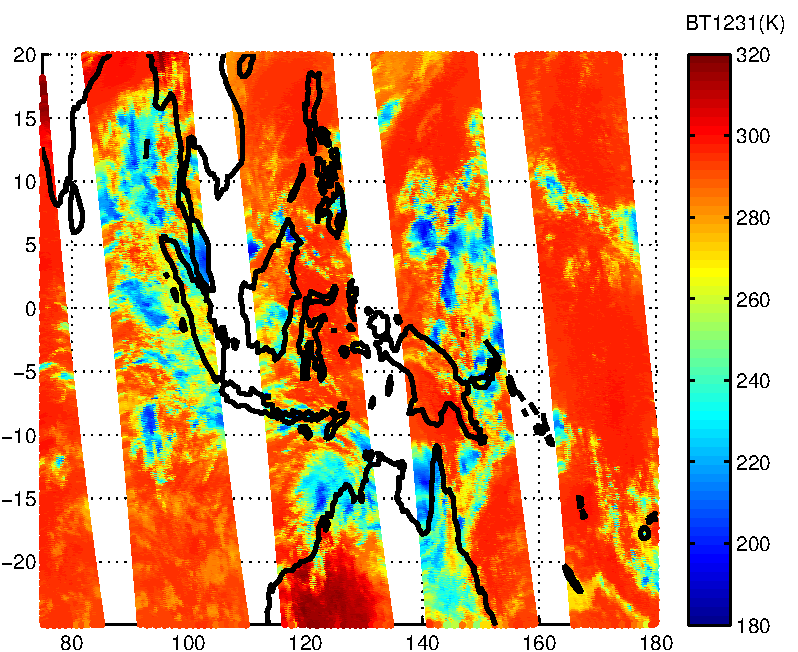
\includegraphics[width=20cm, bb=0 0 1200 900]{FIGS/dcc_twp_obs}
%%\noindent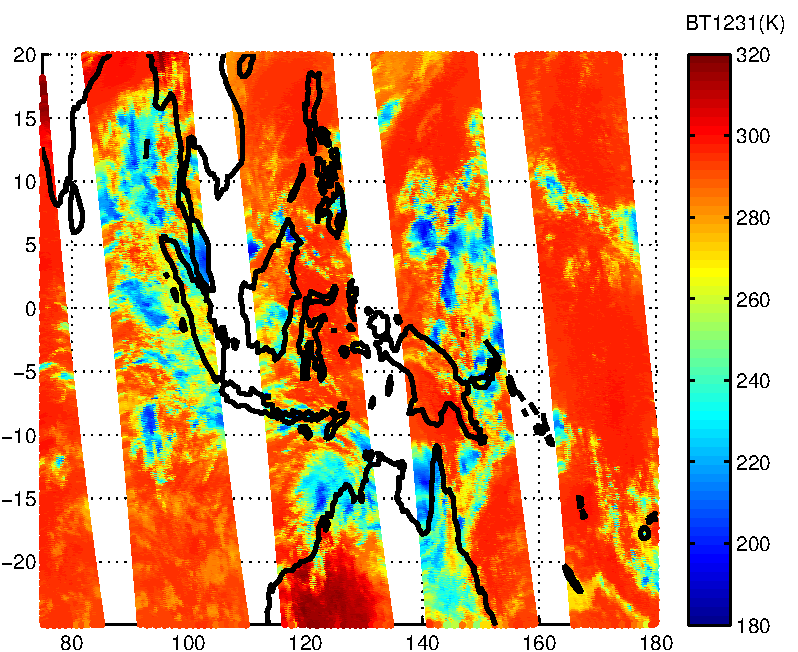
\includegraphics[width=20pc]{FIGS/dcc_twp_obs}
%\caption{Zoom in of the Tropical West Pacific, showing AIRS BT1231 \wn observations in a region with
%deep convection}
%\label{dcc_obs}
%\end{minipage}
%        \hfill{}
%\begin{minipage}[r]{1.0\columnwidth}
%   \centering
%   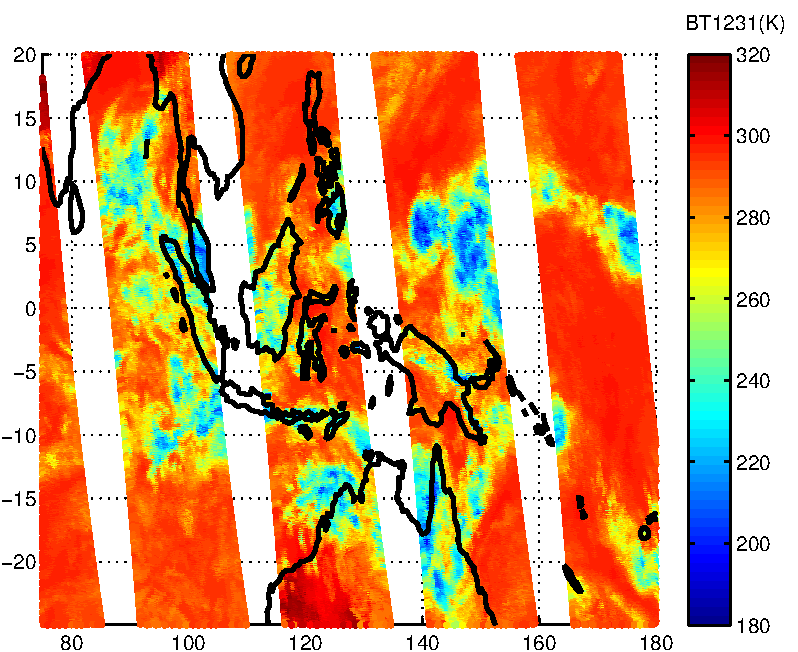
\includegraphics[width=20cm, bb=0 0 1200 900]{FIGS/dcc_twp_sarta}
%\caption{Zoom in of the Tropical West Pacific, showing SARTA 2S BT1231 \wn calculations in a region where 
%deep convection happens}
%\label{dcc_sarta}
%\end{minipage}
%\end{figure*}

For the DCC observations, the 300 mb ECMWF $(u,v)$ wind speeds from
the NWP model showed the convection regions moving westward at
approximately 36 km/h.  The NWP fields used for eg Granule 039 were
forecast on average 0.8 hours before the AIRS overpass, which would
move the convective cells about 30 km (1/3 \mydeg) westward ond
roughly overlay the observed DCC.

Figure \ref{dcc_pdf} shows the observed and calculated BT1231 pdfs for
observations in the Tropical West Pacific. The correlation between the
observed and both of the calculated pdfs is about 0.65. The y-axis is plotted
on a logarithmic scale, to show the under-representation of
deep convective clouds (cold top) in the simulations below about 245 K 
(thin gray vertical line).

\begin{figure}[h]
\noindent\includegraphics[width=20pc]{FIGS/ecm_cloudBT1231_gev_dcc}
\caption{PDFs of the Tropical West Pacific, showing observations and
calculations in a region where deep convection happens. The vertical
gray line shows where the observations and calculations begin to deviate.}
\label{dcc_pdf} 
\end{figure}

\subsubsection{Magnitudes and Timings of Vertical Wind velocities in the TWP}

Convective organization is very complex and is represented by
parametrizations in NWP models; this may lead to a coupling of the
diurnal convective cycle to the diurnal solar cycle, which causes
convection in these models to often start too early in the morning and
be over too soon, especially for precipitating systems \citep{inn:13}.

For cloud tops to reach close to, or past, the tropopause, one would
expect the model fields to show evidence of upwelling vertical
velocities at higher altitudes. An examination of the $\omega$ fields
showed that on average where the biases were small (ie between -20 K
and 0 K), the vertical velocities at both the 300 mb and 500 mb
pressure levels were negative ($\sim$ -2 Pa/s at 300 mb), while for
larger biases the velocities were closer to zero. Examination of
vertical velocities as a function of analysis/forecast timestep (every 3 hours for
March 11, 2011) confirmed that the FOVS with the smallest bias had the
largest upward  $\omega_{500}$  vertical velocities ((as large as -7 Pa/second)
while those with large biases had close to zero vertical velocities at any time. 
These results suggest on average there was not enough convection in the
model and/or started too late to produce the observed number of DCC
clouds.

\subsubsection{DCC Radiative Forcing}

Averaged over the same 733 DCC observations for granule 039,
the mean observed cloud forcing at 1231 \wn is 59.47 $\pm$ 2.17
mW/$m^2$/sr/\wn, while that due to the SARTA 2S and PCRTM MRO
calculations are 41.24 $\pm$ 11.33 and 39.44 $\pm$ 12.65 mW/$m^2$/sr/\wn
respectively.

We then computed the length scales for the observed and calculated cloud 
forcings, shown in Figure \ref{dcc_cldforc}. This figure was produced as follows : 
\begin{itemize}
  \item starting at the center of the  granule (along track and cross track indices = 67,68 and
        45,46 respectively) we averaged the observed and calculated 1231 \wn cloud forcing,
  \item we then fanned out from the center, widening the along and cross track indices by 4 each time 
        (to eg along track indices 65,70 and cross track indices 43,48) and averaging the
        observed and calculated cloud forcing at each iteration;
  \item assuming each pixel had a size of 20 km, the grid size averaging distance is then $\sim$ (difference 
        in cross track extreme indices) $\times$ 20 km
\end{itemize}

The observed AIRS cloud forcing started out at 45 radiance units for
the smallest (40 km) grid size average, while that from the PCRTM and
SARTA calculations were about 23 and 33 radiance units respectively.
Note these differ from the ones in the previous paragraph since those
numbers were averages over the actual DCCs.  The observed forcing then
decreased as the averaging length/area increased, finally reaching
$\sim$ 20.38 $\pm$ 17.20 units for the observed forcing averaged over
the entire granule (about 2000 km), compared to the SARTA and PCRTM
cloud forcings of 20.02 $\pm$ 15.61 and 17.96 $\pm$ 14.32 units
respectively.  Granule 039 had DCC over ocean and land, and as seen
from Figure \ref{dcc_pdf} there were differences between the SARTA 2S
and PCRTM simulations. Though not shown here, this reduction is seen
more clearly from the (observed-calculated) cloud forcing, from which
the $e$-folding distance is roughly 350 km and becomes roughly the same (35
radiance uniits) for both observations and calculations by $\sim$ 750
km averaging size, which is a typical length scale of cloud clusters
(see for example Figure 3 on pg 53 of \cite{vonStorch:99}).

\begin{figure}[h]
\noindent\includegraphics[width=20pc]{FIGS/ecm_cloudBT1231_gev_dcc_cloudforceVSgridsize}
\caption{Cloud forcing as a function of averaged distance for regions with DCC}
\label{dcc_cldforc}
\end{figure}

\section{Conclusions} 

Millions of observed low noise, accurate infrared top-of-atmosphere
radiances from the AIRS instrument were used to assess
state-of-the-art ECMWF NWP geophysical and cloud parameters via
radiative closure. Two different scattering radiative transfer models
were used, along with two different cloud representation schemes.  For
scenes passed through a stringent clear sky filter, AIRS observations
are slightly cooler than the simulated BT 1231 temperatures, probably
due to a combination of higher SST skin temperature model fields
and/or underestimating column water amounts.  Probability distribution
functions for the 1231 \wn channel constructed from observations and
simulations yield consistent moments (mean, standard deviation,
skewness and kurtosis) and other statistical quantities such as maxima
and minima. Under these clear sky conditions, the two models yield
similar synthetic spectra in the window region, with biases typically less
than -0.5 K; on average a +10\% column water vapor and ozone adjustment, 
together with a -0.3K SST adjustment, should be sufficent to reduce the biases
down to AIRS noise levels. 

Looking at the all-sky observations, statistically, the SARTA 2S
scheme produced very similar pdfs to those coming from the PCRTM MRO
scheme, both of which agreed in general with the AIRS
observations. However in the polar regions and in areas where there
are low MBL clouds, the MRO scheme was slighly superior to the SARTA
2S scheme. For deep convection, there were many instances when no
significant convection was initiated in the model; there are some
instances when convection is initiated after the observation, or is
too weak. Assuming accurate SSTs, the cloudtops/height of temperature
inversion appeared to be about 1/3 km (2-3 K) too low in regions of
shallow convection. In terms of Brightness Temperatures, the spectral
cloud forcing was about 10 K in the window regions, and decreasing from
that number as the channel weighting functions peak higher in the
atmosphere. The spectral bias between all-sky AIRS observations and
calculations is on the order of 2-3K, with smaller biases and 
less variability in the higher altitude channels. 
 
By reducing a cloud profile
to an optimally placed slab representation, the SARTA 2S model uses
only four subcolumns to compute a radiance, and consequentially is
about an order of magnitude faster than other schemes such as Maximum
Random Overlap. 
AIRS L2 algorithm already retrieves information for 2 cloud decks
\citep{kah:08}, and this paper demonstrates the applicability of a two
slab layer scattering model for use in operational AIRS L2 retrievals,
where the high spectral resolution of current infrared sounders
translates to improved vertical resolution of moisture, temperature
and cloud fields.  The radiances generated by the SARTA 2S model could
be used as a training set for a regression based retrieval, or
directly in a physically based retrieval.  An information content
study of all-sky AIRS radiances suggests there typically are about 4-6
pieces of cloud water and ice profile information, implying a TwoSlab
prescription (cloud amount and cloud top for each of high and low
cloud decks) should be adequate for retrieval purposes. The model
could also be used in radiative closure validations while diagnosing
physical parametrization schemes in NWPs, and for climate studies
comparing the 12+ years of AIRS (and other hyperspectral) data record
against all-sky simulations.  Future refinement of cloud
representation models within scattering RTAs could improve the amount
of infrared radiance data assimilated into NWPs to extend over all
regions, rather than clear-sky regions only.

%%%%%%%%%%%%%%%%%%%%%%%%%%%%%%%%%%%%%%%%%%%%%%%%%%%%%%%%%%%%%%%%%%%%%%%%
\section{Appendix} 

The following tables shows the night time statistics for the AIRS
observations versus SARTA and PCRTM simulations.  Table
\ref{table:night_all2} shows comparisons between all-sky AIRS
observations and clear-sky SARTA/PCRTM calculations, thus painting a
spectral picture of the cloud forcing (albeit with a negative
sign). The cloud forcing is largest (on the order of 10 K) in the
thermal infrared windows, and least in the high altitude channels.

\begin{center}
\begin{table*}[ht]
{\footnotesize
\hfill{}
\begin{tabular}{c|ccc|ccc|ccc} % centered columns (4 columns)
Wavenumber & AIRS   & PCRTM    & SARTA    & AIRS   & PCRTM    & SARTA    & AIRS   & PCRTM    & SARTA \\
cm-1       & OBS (K)& BIAS (K) & BIAS (K) & OBS (K)& BIAS (K) & BIAS (K) & OBS (K)& BIAS (K) & BIAS (K) \\
           &        & TRP      &          &        & MIDLAT   &          &        & POLAR    &       \\
\hline
659.23 & 217.7$\pm$1.7 &  1.0$\pm$0.8 &  0.3$\pm$0.7 & 222.4$\pm$3.2 &  0.6$\pm$0.7 &  0.3$\pm$0.7 & 216.5$\pm$9.7 &  0.4$\pm$0.7 &  0.3$\pm$0.7 \\ 
662.45 & 233.1$\pm$1.2 & -0.5$\pm$0.7 & -0.1$\pm$0.6 & 232.2$\pm$3.5 & -0.4$\pm$0.6 & -0.2$\pm$0.6 & 227.6$\pm$5.3 & -0.4$\pm$0.7 & -0.1$\pm$0.7 \\ 
701.26 & 221.5$\pm$2.9 & -1.7$\pm$2.3 & -0.9$\pm$2.3 & 222.5$\pm$2.8 & -0.7$\pm$0.9 & -0.3$\pm$0.9 & 217.6$\pm$8.3 & -0.4$\pm$0.6 & -0.1$\pm$0.5 \\ 
728.05 & 258.2$\pm$10.2 & -5.6$\pm$9.5 & -4.6$\pm$9.5 & 249.0$\pm$8.9 & -6.0$\pm$7.1 & -5.2$\pm$7.1 & 238.5$\pm$6.9 & -5.0$\pm$5.1 & -4.6$\pm$5.1 \\ 
740.89 & 238.1$\pm$5.5 & -2.6$\pm$4.9 & -2.1$\pm$4.9 & 233.6$\pm$4.2 & -1.9$\pm$2.9 & -1.5$\pm$2.9 & 227.7$\pm$5.4 & -1.5$\pm$2.0 & -1.3$\pm$2.0 \\ 
754.26 & 259.1$\pm$10.4 & -4.9$\pm$8.9 & -4.1$\pm$8.9 & 251.5$\pm$8.9 & -5.6$\pm$7.1 & -4.9$\pm$7.1 & 242.1$\pm$6.8 & -5.5$\pm$5.8 & -5.2$\pm$5.7 \\ 
790.23 & 282.1$\pm$16.3 & -9.8$\pm$15.3 & -9.5$\pm$15.2 & 267.7$\pm$15.0 & -13.1$\pm$13.1 & -13.0$\pm$13.1 & 249.6$\pm$10.7 & -10.4$\pm$10.5 & -11.4$\pm$10.0 \\ 
791.65* & 266.8$\pm$15.0 & -6.9$\pm$14.4 & -6.2$\pm$14.4 & 256.3$\pm$15.1 & -9.2$\pm$13.9 & -8.6$\pm$13.9 & 243.7$\pm$14.4 & -8.4$\pm$14.2 & -8.3$\pm$14.1 \\ 
\hline
822.26 & 283.2$\pm$16.4 & -10.0$\pm$15.5 & -9.6$\pm$15.5 & 268.4$\pm$15.2 & -13.4$\pm$13.3 & -13.2$\pm$13.3 & 250.1$\pm$10.8 & -10.8$\pm$10.6 & -11.6$\pm$10.1 \\ 
899.87 & 284.6$\pm$16.4 & -9.8$\pm$15.7 & -9.7$\pm$15.7 & 269.2$\pm$15.2 & -13.3$\pm$13.3 & -13.3$\pm$13.3 & 250.5$\pm$10.8 & -11.5$\pm$10.1 & -11.7$\pm$10.0 \\ 
960.95 & 285.7$\pm$16.1 & -9.5$\pm$15.6 & -9.5$\pm$15.6 & 270.0$\pm$15.0 & -12.8$\pm$13.1 & -12.8$\pm$13.1 & 251.2$\pm$10.7 & -11.2$\pm$9.7 & -11.1$\pm$9.7 \\ 
961.35 & 285.7$\pm$16.1 & -9.5$\pm$15.6 & -9.5$\pm$15.6 & 269.9$\pm$15.0 & -12.8$\pm$13.1 & -12.8$\pm$13.1 & 251.2$\pm$10.7 & -11.2$\pm$9.6 & -11.0$\pm$9.7 \\ 
\hline
999.98 & 280.7$\pm$14.4 & -8.7$\pm$13.8 & -8.5$\pm$13.8 & 265.4$\pm$13.6 & -11.8$\pm$11.5 & -11.6$\pm$11.5 & 248.1$\pm$9.7 & -10.2$\pm$8.5 & -10.0$\pm$8.5 \\ 
1008.62 & 277.3$\pm$13.5 & -8.7$\pm$13.1 & -8.5$\pm$13.1 & 261.3$\pm$12.9 & -11.1$\pm$10.5 & -10.9$\pm$10.5 & 244.4$\pm$9.2 & -9.4$\pm$7.5 & -9.1$\pm$7.5 \\ 
1014.75 & 271.0$\pm$11.9 & -8.1$\pm$11.1 & -7.7$\pm$11.1 & 256.4$\pm$11.7 & -10.0$\pm$8.9 & -9.7$\pm$8.8 & 240.5$\pm$8.7 & -8.4$\pm$6.4 & -8.0$\pm$6.4 \\ 
1024.09 & 266.4$\pm$10.9 & -8.0$\pm$10.3 & -7.5$\pm$10.3 & 251.1$\pm$10.9 & -9.0$\pm$7.6 & -8.6$\pm$7.6 & 235.4$\pm$8.8 & -7.1$\pm$5.1 & -6.6$\pm$5.1 \\ 
1033.14 & 264.3$\pm$10.3 & -7.9$\pm$9.7 & -7.3$\pm$9.7 & 249.7$\pm$10.4 & -8.7$\pm$7.1 & -8.2$\pm$7.1 & 234.6$\pm$8.6 & -6.8$\pm$4.8 & -6.3$\pm$4.7 \\ 
1046.07 & 267.2$\pm$11.1 & -7.9$\pm$10.6 & -7.3$\pm$10.6 & 251.8$\pm$11.0 & -9.0$\pm$7.9 & -8.4$\pm$7.9 & 235.7$\pm$9.1 & -6.9$\pm$5.3 & -6.4$\pm$5.3 \\ 
\hline
1129.46 & 285.3$\pm$15.6 & -9.4$\pm$15.3 & -9.4$\pm$15.3 & 269.0$\pm$14.6 & -12.6$\pm$12.6 & -12.6$\pm$12.6 & 250.5$\pm$10.3 & -10.7$\pm$9.4 & -10.6$\pm$9.4 \\ 
1226.54 & 281.0$\pm$14.5 & -8.0$\pm$13.2 & -7.6$\pm$13.2 & 268.0$\pm$13.8 & -11.6$\pm$11.8 & -11.5$\pm$11.8 & 250.6$\pm$10.2 & -10.7$\pm$9.3 & -10.7$\pm$9.2 \\ 
1231.19 & 285.4$\pm$15.7 & -9.6$\pm$15.3 & -9.4$\pm$15.3 & 269.3$\pm$14.7 & -12.9$\pm$12.8 & -12.9$\pm$12.8 & 250.7$\pm$10.4 & -11.2$\pm$9.6 & -11.1$\pm$9.6 \\ 
\hline
1329.61 & 267.1$\pm$11.9 & -4.3$\pm$8.8 & -4.0$\pm$8.8 & 259.1$\pm$10.4 & -5.9$\pm$7.6 & -5.6$\pm$7.6 & 248.1$\pm$7.8 & -6.7$\pm$6.5 & -6.5$\pm$6.5 \\ 
1344.15 & 269.9$\pm$12.4 & -4.8$\pm$9.5 & -4.5$\pm$9.5 & 261.4$\pm$11.1 & -6.7$\pm$8.5 & -6.4$\pm$8.5 & 249.0$\pm$8.5 & -7.6$\pm$7.2 & -7.4$\pm$7.2 \\ 
1387.61 & 240.6$\pm$7.8 & -2.3$\pm$3.9 & -0.9$\pm$3.9 & 235.8$\pm$5.3 & -1.9$\pm$2.5 & -0.6$\pm$2.5 & 231.5$\pm$4.5 & -1.7$\pm$2.1 & -0.6$\pm$2.1 \\ 
1413.85 & 263.2$\pm$11.8 & -3.0$\pm$7.7 & -3.2$\pm$7.7 & 255.8$\pm$9.7 & -3.2$\pm$6.1 & -3.5$\pm$6.2 & 247.6$\pm$7.1 & -3.7$\pm$5.4 & -3.9$\pm$5.4 \\ 
1419.57 & 230.3$\pm$5.9 & -1.4$\pm$2.6 & -0.3$\pm$2.7 & 228.0$\pm$3.8 & -0.9$\pm$1.6 & -0.1$\pm$1.5 & 224.4$\pm$4.7 & -0.8$\pm$1.2 & -0.1$\pm$1.2 \\ 
1421.87 & 256.1$\pm$11.1 & -2.9$\pm$6.3 & -2.1$\pm$6.3 & 249.0$\pm$8.4 & -2.7$\pm$4.6 & -2.0$\pm$4.6 & 242.9$\pm$6.3 & -2.6$\pm$4.0 & -2.0$\pm$4.0 \\ 
1463.15 & 249.3$\pm$10.1 & -2.6$\pm$5.2 & -1.4$\pm$5.2 & 242.4$\pm$7.2 & -2.2$\pm$3.5 & -1.1$\pm$3.5 & 236.9$\pm$5.5 & -2.0$\pm$2.9 & -1.1$\pm$2.9 \\ 
1560.75 & 229.3$\pm$6.2 & -0.9$\pm$2.8 & -0.2$\pm$2.8 & 226.7$\pm$4.1 & -0.4$\pm$1.7 & -0.0$\pm$1.7 & 222.7$\pm$5.1 & -0.4$\pm$1.5 & -0.0$\pm$1.5 \\ 
\hline
2182.16 & 278.0$\pm$12.6 & -7.6$\pm$12.4 & -6.6$\pm$12.3 & 263.6$\pm$12.2 & -9.9$\pm$10.2 & -9.0$\pm$10.2 & 247.8$\pm$8.6 & -8.6$\pm$7.6 & -7.8$\pm$7.5 \\ 
2183.06 & 276.3$\pm$12.3 & -7.7$\pm$12.1 & -6.1$\pm$12.1 & 262.1$\pm$12.0 & -9.6$\pm$9.9 & -8.2$\pm$9.9 & 246.7$\pm$8.3 & -8.1$\pm$7.3 & -7.1$\pm$7.1 \\ 
2183.97 & 276.4$\pm$12.3 & -7.4$\pm$12.0 & -6.4$\pm$12.0 & 262.6$\pm$11.9 & -9.6$\pm$9.9 & -8.7$\pm$9.9 & 247.1$\pm$8.3 & -8.2$\pm$7.4 & -7.6$\pm$7.3 \\ 
2193.08 & 271.5$\pm$11.4 & -7.0$\pm$11.1 & -5.8$\pm$11.1 & 258.2$\pm$11.0 & -8.7$\pm$9.0 & -7.6$\pm$8.9 & 243.7$\pm$7.7 & -7.2$\pm$6.6 & -6.4$\pm$6.4 \\ 
2202.26 & 264.9$\pm$10.3 & -6.7$\pm$9.9 & -5.0$\pm$9.9 & 252.3$\pm$9.8 & -7.5$\pm$7.6 & -5.9$\pm$7.6 & 239.2$\pm$7.2 & -5.8$\pm$5.4 & -4.7$\pm$5.2 \\ 
2390.82 & 268.4$\pm$10.0 & -5.4$\pm$9.7 & -4.4$\pm$9.6 & 255.9$\pm$9.9 & -6.3$\pm$7.5 & -5.7$\pm$7.5 & 242.9$\pm$7.1 & -4.8$\pm$5.4 & -4.7$\pm$5.3 \\ 
\hline
2418.56 & 282.7$\pm$12.9 & -7.6$\pm$12.9 & -7.0$\pm$12.8 & 266.2$\pm$12.7 & -10.0$\pm$10.4 & -9.5$\pm$10.4 & 249.1$\pm$8.6 & -8.4$\pm$7.7 & -7.9$\pm$7.6 \\ 
2603.38 & 289.3$\pm$13.6 & -8.0$\pm$13.6 & -8.0$\pm$13.7 & 271.3$\pm$13.8 & -11.6$\pm$11.5 & -11.6$\pm$11.5 & 251.7$\pm$10.0 & -10.5$\pm$8.7 & -10.4$\pm$8.8 \\ 
2607.60 & 286.9$\pm$13.1 & -6.9$\pm$12.6 & -7.2$\pm$12.6 & 270.9$\pm$13.4 & -10.8$\pm$11.0 & -10.9$\pm$11.1 & 251.8$\pm$9.9 & -10.2$\pm$8.6 & -10.2$\pm$8.6 \\ 
2616.09 & 289.9$\pm$13.7 & -8.0$\pm$13.7 & -8.1$\pm$13.7 & 271.7$\pm$13.8 & -11.7$\pm$11.6 & -11.7$\pm$11.6 & 251.9$\pm$10.1 & -10.6$\pm$8.8 & -10.5$\pm$8.8 \\ 
2622.50 & 286.7$\pm$13.0 & -6.8$\pm$12.4 & -7.1$\pm$12.5 & 270.8$\pm$13.3 & -10.6$\pm$10.9 & -10.7$\pm$11.0 & 251.8$\pm$9.9 & -10.1$\pm$8.5 & -10.1$\pm$8.5 \\ 
2637.58 & 286.5$\pm$12.9 & -6.7$\pm$12.3 & -7.0$\pm$12.4 & 270.7$\pm$13.2 & -10.4$\pm$10.8 & -10.5$\pm$10.8 & 251.9$\pm$9.8 & -9.9$\pm$8.4 & -9.9$\pm$8.5 \\ 
\hline
\end{tabular}}
\hfill{}
\caption{Night time allsky ocean scenes : cloud forcing ( = obs - clear calcs); all units in Kelvin}
\label{table:night_all2} % is used to refer this table in the text
\end{table*}
\end{center}

%%%%%%%%%%%%%%%%%%%%%%%%%

Table \ref{table:night_allbias2} shows comparisons between all-sky
AIRS observations and all-sky SARTA/PCRTM calculations. The all-sky
biases are larger than the clear-sky biases, due to a combination of
inaccurately representing the cloud fields as represented in the NWP
scheme, and with cloud parametrization problems in the NWP itself. A
dedicated retrieval scheme can be be used to improve the biases. The
791 \wn channel is starred since it occasionally had bad data.

\begin{center}
\begin{table*}[ht]
{\footnotesize
\hfill{}
\begin{tabular}{c|ccc|ccc|ccc} % centered columns (4 columns)
Wavenumber & AIRS   & PCRTM    & SARTA    & AIRS   & PCRTM    & SARTA    & AIRS   & PCRTM    & SARTA \\
cm-1       & OBS (K)& BIAS (K) & BIAS (K) & OBS (K)& BIAS (K) & BIAS (K) & OBS (K)& BIAS (K) & BIAS (K) \\
           &        & TRP      &          &        & MIDLAT   &          &        & POLAR    &       \\
\hline
659.23 & 217.7$\pm$1.7 &  1.0$\pm$0.8 &  0.3$\pm$0.7 & 222.4$\pm$3.2 &  0.6$\pm$0.7 &  0.3$\pm$0.7 & 216.5$\pm$9.7 &  0.4$\pm$0.7 &  0.3$\pm$0.7 \\ 
662.45 & 233.1$\pm$1.2 & -0.5$\pm$0.7 & -0.1$\pm$0.6 & 232.2$\pm$3.5 & -0.4$\pm$0.6 & -0.2$\pm$0.6 & 227.6$\pm$5.3 & -0.4$\pm$0.7 & -0.1$\pm$0.7 \\ 
701.26 & 221.5$\pm$2.9 & -1.1$\pm$2.2 & -0.2$\pm$2.3 & 222.5$\pm$2.8 & -0.5$\pm$0.8 & -0.1$\pm$0.8 & 217.6$\pm$8.3 & -0.3$\pm$0.5 &  0.0$\pm$0.5 \\ 
728.05 & 258.2$\pm$10.2 & -2.3$\pm$8.1 & -0.5$\pm$8.3 & 249.0$\pm$8.9 & -2.5$\pm$5.2 & -1.2$\pm$5.4 & 238.5$\pm$6.9 & -2.0$\pm$3.9 & -1.0$\pm$4.5 \\ 
740.89 & 238.1$\pm$5.5 & -1.1$\pm$4.4 & -0.4$\pm$4.6 & 233.6$\pm$4.2 & -0.9$\pm$2.3 & -0.3$\pm$2.3 & 227.7$\pm$5.4 & -0.6$\pm$1.6 & -0.1$\pm$1.9 \\ 
754.26 & 259.1$\pm$10.4 & -2.0$\pm$7.8 & -0.5$\pm$8.1 & 251.5$\pm$8.9 & -2.4$\pm$5.4 & -1.1$\pm$5.6 & 242.1$\pm$6.8 & -2.2$\pm$4.5 & -1.3$\pm$5.2 \\ 
790.23 & 282.1$\pm$16.3 & -2.9$\pm$12.6 & -1.1$\pm$13.2 & 267.7$\pm$15.0 & -4.6$\pm$9.7 & -3.7$\pm$10.1 & 249.6$\pm$10.7 & -4.7$\pm$7.9 & -4.3$\pm$8.9 \\ 
791.65* & 266.8$\pm$15.0 & -2.6$\pm$12.9 & -0.9$\pm$13.2 & 256.3$\pm$15.1 & -3.9$\pm$12.3 & -2.6$\pm$12.4 & 243.7$\pm$14.4 & -4.1$\pm$13.1 & -3.2$\pm$13.4 \\ 
\hline
822.26 & 283.2$\pm$16.4 & -2.9$\pm$12.8 & -1.1$\pm$13.4 & 268.4$\pm$15.2 & -4.7$\pm$9.8 & -3.6$\pm$10.2 & 250.1$\pm$10.8 & -5.0$\pm$7.9 & -4.3$\pm$9.0 \\ 
899.87 & 284.6$\pm$16.4 & -2.5$\pm$12.9 & -0.9$\pm$13.5 & 269.2$\pm$15.2 & -4.7$\pm$9.8 & -3.6$\pm$10.2 & 250.5$\pm$10.8 & -5.7$\pm$7.7 & -4.4$\pm$9.0 \\ 
960.95 & 285.7$\pm$16.1 & -2.2$\pm$12.8 & -0.7$\pm$13.4 & 270.0$\pm$15.0 & -4.4$\pm$9.7 & -3.2$\pm$10.1 & 251.2$\pm$10.7 & -5.7$\pm$7.4 & -3.9$\pm$8.9 \\ 
961.35 & 285.7$\pm$16.1 & -2.2$\pm$12.7 & -0.7$\pm$13.4 & 269.9$\pm$15.0 & -4.4$\pm$9.7 & -3.2$\pm$10.1 & 251.2$\pm$10.7 & -5.7$\pm$7.4 & -3.8$\pm$8.8 \\ 
\hline
999.98 & 280.7$\pm$14.4 & -2.2$\pm$11.4 & -0.7$\pm$12.0 & 265.4$\pm$13.6 & -4.3$\pm$8.6 & -3.1$\pm$8.9 & 248.1$\pm$9.7 & -5.3$\pm$6.6 & -3.7$\pm$7.9 \\ 
1008.62 & 277.3$\pm$13.5 & -2.3$\pm$10.7 & -0.9$\pm$11.3 & 261.3$\pm$12.9 & -4.1$\pm$7.8 & -3.1$\pm$8.1 & 244.4$\pm$9.2 & -5.0$\pm$5.8 & -3.4$\pm$6.9 \\ 
1014.75 & 271.0$\pm$11.9 & -2.8$\pm$9.2 & -1.4$\pm$9.7 & 256.4$\pm$11.7 & -4.1$\pm$6.6 & -3.0$\pm$6.9 & 240.5$\pm$8.7 & -4.6$\pm$5.0 & -3.2$\pm$5.9 \\ 
1024.09 & 266.4$\pm$10.9 & -2.7$\pm$8.5 & -1.4$\pm$9.0 & 251.1$\pm$10.9 & -3.7$\pm$5.7 & -2.8$\pm$5.9 & 235.4$\pm$8.8 & -4.0$\pm$4.0 & -2.7$\pm$4.7 \\ 
1033.14 & 264.3$\pm$10.3 & -2.9$\pm$8.0 & -1.5$\pm$8.4 & 249.7$\pm$10.4 & -3.8$\pm$5.3 & -2.7$\pm$5.5 & 234.6$\pm$8.6 & -3.9$\pm$3.7 & -2.6$\pm$4.4 \\ 
1046.07 & 267.2$\pm$11.1 & -2.5$\pm$8.7 & -1.1$\pm$9.2 & 251.8$\pm$11.0 & -3.6$\pm$5.9 & -2.5$\pm$6.1 & 235.7$\pm$9.1 & -3.7$\pm$4.1 & -2.4$\pm$4.8 \\ 
\hline
1129.46 & 285.3$\pm$15.6 & -2.1$\pm$12.5 & -0.9$\pm$13.1 & 269.0$\pm$14.6 & -4.3$\pm$9.4 & -3.5$\pm$9.7 & 250.5$\pm$10.3 & -5.4$\pm$7.3 & -3.9$\pm$8.6 \\ 
1226.54 & 281.0$\pm$14.5 & -2.6$\pm$11.1 & -1.1$\pm$11.6 & 268.0$\pm$13.8 & -4.4$\pm$8.9 & -3.4$\pm$9.3 & 250.6$\pm$10.2 & -5.5$\pm$7.2 & -4.1$\pm$8.5 \\ 
1231.19 & 285.4$\pm$15.7 & -2.4$\pm$12.5 & -1.2$\pm$13.0 & 269.3$\pm$14.7 & -4.7$\pm$9.5 & -3.8$\pm$9.8 & 250.7$\pm$10.4 & -5.8$\pm$7.4 & -4.4$\pm$8.7 \\ 
\hline
1329.61 & 267.1$\pm$11.9 & -1.7$\pm$7.9 & -0.6$\pm$8.2 & 259.1$\pm$10.4 & -2.6$\pm$6.0 & -1.5$\pm$6.3 & 248.1$\pm$7.8 & -3.3$\pm$5.2 & -2.0$\pm$6.2 \\ 
1344.15 & 269.9$\pm$12.4 & -2.0$\pm$8.5 & -0.8$\pm$8.8 & 261.4$\pm$11.1 & -2.9$\pm$6.6 & -1.8$\pm$6.9 & 249.0$\pm$8.5 & -3.7$\pm$5.7 & -2.4$\pm$6.8 \\ 
1387.61 & 240.6$\pm$7.8 & -1.4$\pm$3.9 &  0.2$\pm$4.1 & 235.8$\pm$5.3 & -1.3$\pm$2.3 &  0.1$\pm$2.4 & 231.5$\pm$4.5 & -1.1$\pm$1.9 &  0.2$\pm$2.1 \\ 
1413.85 & 263.2$\pm$11.8 & -1.0$\pm$7.1 & -0.7$\pm$7.3 & 255.8$\pm$9.7 & -1.3$\pm$5.1 & -0.7$\pm$5.4 & 247.6$\pm$7.1 & -1.3$\pm$4.3 & -0.5$\pm$5.3 \\ 
1419.57 & 230.3$\pm$5.9 & -0.9$\pm$2.7 &  0.3$\pm$2.8 & 228.0$\pm$3.8 & -0.7$\pm$1.5 &  0.2$\pm$1.5 & 224.4$\pm$4.7 & -0.5$\pm$1.2 &  0.2$\pm$1.2 \\ 
1421.87 & 256.1$\pm$11.1 & -1.4$\pm$6.0 & -0.3$\pm$6.2 & 249.0$\pm$8.4 & -1.4$\pm$4.0 & -0.2$\pm$4.2 & 242.9$\pm$6.3 & -1.1$\pm$3.3 &  0.2$\pm$4.0 \\ 
1463.15 & 249.3$\pm$10.1 & -1.4$\pm$5.1 &  0.0$\pm$5.3 & 242.4$\pm$7.2 & -1.4$\pm$3.2 & -0.0$\pm$3.3 & 236.9$\pm$5.5 & -1.1$\pm$2.6 &  0.2$\pm$3.0 \\ 
1560.75 & 229.3$\pm$6.2 & -0.4$\pm$2.9 &  0.3$\pm$3.0 & 226.7$\pm$4.1 & -0.3$\pm$1.7 &  0.2$\pm$1.7 & 222.7$\pm$5.1 & -0.2$\pm$1.5 &  0.2$\pm$1.5 \\ 
\hline
2182.16 & 278.0$\pm$12.6 & -2.5$\pm$10.1 & -0.6$\pm$10.4 & 263.6$\pm$12.2 & -3.9$\pm$7.6 & -2.4$\pm$7.8 & 247.8$\pm$8.6 & -4.6$\pm$5.8 & -2.7$\pm$6.7 \\ 
2183.06 & 276.3$\pm$12.3 & -2.7$\pm$9.9 & -0.3$\pm$10.2 & 262.1$\pm$12.0 & -3.8$\pm$7.3 & -1.9$\pm$7.5 & 246.7$\pm$8.3 & -4.3$\pm$5.5 & -2.2$\pm$6.3 \\ 
2183.97 & 276.4$\pm$12.3 & -2.6$\pm$9.9 & -0.7$\pm$10.1 & 262.6$\pm$11.9 & -3.9$\pm$7.4 & -2.3$\pm$7.5 & 247.1$\pm$8.3 & -4.4$\pm$5.6 & -2.6$\pm$6.5 \\ 
2193.08 & 271.5$\pm$11.4 & -2.6$\pm$9.2 & -0.6$\pm$9.4 & 258.2$\pm$11.0 & -3.6$\pm$6.6 & -1.9$\pm$6.8 & 243.7$\pm$7.7 & -3.7$\pm$4.9 & -1.9$\pm$5.6 \\ 
2202.26 & 264.9$\pm$10.3 & -2.8$\pm$8.2 & -0.3$\pm$8.4 & 252.3$\pm$9.8 & -3.3$\pm$5.5 & -1.3$\pm$5.7 & 239.2$\pm$7.2 & -3.0$\pm$3.9 & -1.0$\pm$4.5 \\ 
2390.82 & 268.4$\pm$10.0 & -2.2$\pm$8.0 & -0.5$\pm$8.2 & 255.9$\pm$9.9 & -2.7$\pm$5.5 & -1.4$\pm$5.6 & 242.9$\pm$7.1 & -2.4$\pm$3.9 & -1.2$\pm$4.6 \\ 
\hline
2418.56 & 282.7$\pm$12.9 & -2.1$\pm$10.6 & -1.0$\pm$10.8 & 266.2$\pm$12.7 & -3.9$\pm$7.8 & -2.9$\pm$7.9 & 249.1$\pm$8.6 & -4.7$\pm$5.9 & -2.9$\pm$6.7 \\ 
2603.38 & 289.3$\pm$13.6 & -1.7$\pm$11.3 & -1.6$\pm$11.5 & 271.3$\pm$13.8 & -4.3$\pm$8.9 & -4.4$\pm$9.0 & 251.7$\pm$10.0 & -6.4$\pm$7.2 & -5.1$\pm$8.0 \\ 
2607.60 & 286.9$\pm$13.1 & -1.5$\pm$10.5 & -1.4$\pm$10.8 & 270.9$\pm$13.4 & -4.1$\pm$8.6 & -4.0$\pm$8.7 & 251.8$\pm$9.9 & -6.2$\pm$7.1 & -5.0$\pm$8.0 \\ 
2616.09 & 289.9$\pm$13.7 & -1.6$\pm$11.3 & -1.6$\pm$11.6 & 271.7$\pm$13.8 & -4.3$\pm$9.0 & -4.5$\pm$9.0 & 251.9$\pm$10.1 & -6.4$\pm$7.2 & -5.2$\pm$8.1 \\ 
2622.50 & 286.7$\pm$13.0 & -1.5$\pm$10.4 & -1.4$\pm$10.6 & 270.8$\pm$13.3 & -4.0$\pm$8.6 & -3.9$\pm$8.6 & 251.8$\pm$9.9 & -6.2$\pm$7.0 & -4.9$\pm$7.9 \\ 
2637.58 & 286.5$\pm$12.9 & -1.4$\pm$10.4 & -1.3$\pm$10.6 & 270.7$\pm$13.2 & -3.9$\pm$8.5 & -3.8$\pm$8.6 & 251.9$\pm$9.8 & -6.0$\pm$7.0 & -4.8$\pm$7.8 \\ 
\hline
\end{tabular}}
\hfill{}
\caption{Night time allsky ocean biases; all units in Kelvin}
\label{table:night_allbias2} % is used to refer this table in the text
\end{table*}
\end{center}

%%%%%%%%%%%%%%%%%%%%%%%%%%%%%%%%%%%%%%%%%%%%%%%%%%%%%%%%%%%%%%%%%%%%%%%%
\begin{acknowledgments} 
We acknowledge the use of ECMWF model fields
to compute radiances. The hardware used in the computational studies
is part of the UMBC High Performance Computing Facility (HPCF). The
facility is supported by the U.S. National Science Foundation through
the MRI program (grant nos.~CNS--0821258 and CNS--1228778) and the
SCREMS program (grant no.~DMS--0821311), with additional substantial
support from the University of Maryland, Baltimore County (UMBC). See
\verb+www.umbc.edu/hpcf+ for more information on HPCF and the projects
using its resources.

\end{acknowledgments}

\bibliographystyle{agu} 
\bibliography{/home/sergio/PAPERS/BIB/atmspec2002} 

\end{article}
\end{document}

LocalWords:  DeSouza Machado Strow Hannon Schou affil JCET Liu
LocalWords:  forcings
